\documentclass[
    11pt, 
    english, 
    singlespacing,
    headsepline,
    openany
]{MastersDoctoralThesis} 

\usepackage[utf8]{inputenc} % Required for inputting international characters
\usepackage[T1]{fontenc} % Output font encoding for international characters
\usepackage{caption}
% \usepackage{fncychap}
\usepackage{mathpazo} % Use the Palatino font by default
\usepackage{minitoc}
\usepackage[backend=biber,style=ieee,natbib=true]{biblatex} % Use the bibtex backend with the authoryear citation style (which resembles APA)

\addbibresource{refers.bib} % The filename of the bibliography

\usepackage{graphicx}
\usepackage{float}
\graphicspath{ {./Images/} }

\usepackage[autostyle=true]{csquotes} % Required to generate language-dependent quotes in the bibliography
\usepackage{lipsum} 
\usepackage{tabularx}
%----------------------------------------------------------------------------------------
%	MARGIN SETTINGS
%----------------------------------------------------------------------------------------

\geometry{
	paper=a4paper, % Change to letterpaper for US letter
	inner=2.5cm, % Inner margin
	outer=3.8cm, % Outer margin
	bindingoffset=.5cm, % Binding offset
	top=1.5cm, % Top margin
	bottom=1.5cm, % Bottom margin
	%showframe, % Uncomment to show how the type block is set on the page
}

%----------------------------------------------------------------------------------------
%	THESIS INFORMATION
%----------------------------------------------------------------------------------------

\thesistitle{3D Reconstruction of Video Sign Language Dictionaries} % Your thesis title, this is used in the title and abstract, print it elsewhere with \ttitle
\supervisor{Maksym \textsc{Davydov}} % Your supervisor's name, this is used in the title page, print it elsewhere with \supname
\examiner{} % Your examiner's name, this is not currently used anywhere in the template, print it elsewhere with \examname
\degree{Master of Science} % Your degree name, this is used in the title page and abstract, print it elsewhere with \degreename
\author{Roman \textsc{Riazantsev}} % Your name, this is used in the title page and abstract, print it elsewhere with \authorname
\addresses{} % Your address, this is not currently used anywhere in the template, print it elsewhere with \addressname

\subject{Data Science} % Your subject area, this is not currently used anywhere in the template, print it elsewhere with \subjectname
\keywords{} % Keywords for your thesis, this is not currently used anywhere in the template, print it elsewhere with \keywordnames
\university{\href{http://www.ucu.edu.ua}{Ukrainian Catholic University}} % Your university's name and URL, this is used in the title page and abstract, print it elsewhere with \univname
\department{\href{http://department.university.com}{Faculty of Applied Sciences}} % Your department's name and URL, this is used in the title page and abstract, print it elsewhere with \deptname
\group{\href{http://researchgroup.university.com}{Department of Computer Sciences}} % Your research group's name and URL, this is used in the title page, print it elsewhere with \groupname
\faculty{\href{http://faculty.university.com}{}} % Your faculty's name and URL, this is used in the title page and abstract, print it elsewhere with \facname

\AtBeginDocument{
\hypersetup{pdftitle=\ttitle} % Set the PDF's title to your title
\hypersetup{pdfauthor=\authorname} % Set the PDF's author to your name
\hypersetup{pdfkeywords=\keywordnames} % Set the PDF's keywords to your keywords
}

\newcolumntype{b}{X}
\newcolumntype{s}{>{\hsize=.2\hsize}X}

\begin{document}
\frontmatter % Use roman page numbering style (i, ii, iii, iv...) for the pre-content pages

\pagestyle{plain} % Default to the plain heading style until the thesis style is called for the body content

%----------------------------------------------------------------------------------------
%	TITLE PAGE
%----------------------------------------------------------------------------------------

\begin{titlepage}
\begin{center}

\vspace*{.06\textheight}
{\scshape\LARGE \univname\par}\vspace{1.5cm} % University name
\textsc{\Large Master Thesis}\\[0.5cm] % Thesis type

\HRule \\[0.4cm] % Horizontal line
{\huge \bfseries \ttitle\par}\vspace{0.4cm} % Thesis title
\HRule \\[1.5cm] % Horizontal line
 
\begin{minipage}[t]{0.4\textwidth}
\begin{flushleft} \large
\emph{Author:}\\
\href{http://www.johnsmith.com}{\authorname} % Author name - remove the \href bracket to remove the link
\end{flushleft}
\end{minipage}
\begin{minipage}[t]{0.4\textwidth}
\begin{flushright} \large
\emph{Supervisor:} \\
\href{http://www.jamessmith.com}{\supname} % Supervisor name - remove the \href bracket to remove the link  
\end{flushright}
\end{minipage}\\[2cm]
 
\vfill

\large \textit{A thesis submitted in fulfillment of the requirements\\ for the degree of \degreename}\\[0.3cm] % University requirement text
\textit{in the}\\[0.4cm]
\groupname\\\deptname\\[2cm] % Research group name and department name
 
\vfill

\includegraphics[height=5cm]{UCU-Apps.png} % University/department logo - uncomment to place it

\vfill
{\large Lviv 2020}\\[4cm] % Date
 
\vfill
\end{center}
\end{titlepage}

%----------------------------------------------------------------------------------------
%	DECLARATION PAGE
%----------------------------------------------------------------------------------------

\begin{declaration}
\addchaptertocentry{\authorshipname} % Add the declaration to the table of contents
\noindent I, \authorname, declare that this thesis titled, \enquote{\ttitle} and the work presented in it are my own. I confirm that:

\begin{itemize} 
\item This work was done wholly or mainly while in candidature for a research degree at this University.
\item Where any part of this thesis has previously been submitted for a degree or any other qualification at this University or any other institution, this has been clearly stated.
\item Where I have consulted the published work of others, this is always clearly attributed.
\item Where I have quoted from the work of others, the source is always given. With the exception of such quotations, this thesis is entirely my own work.
\item I have acknowledged all main sources of help.
\item Where the thesis is based on work done by myself jointly with others, I have made clear exactly what was done by others and what I have contributed myself.\\
\end{itemize}
 
\noindent Signed:\\
\rule[0.5em]{25em}{0.5pt} % This prints a line for the signature
 
\noindent Date:\\
\rule[0.5em]{25em}{0.5pt} % This prints a line to write the date
\end{declaration}

\cleardoublepage

%----------------------------------------------------------------------------------------
%	QUOTATION PAGE
%----------------------------------------------------------------------------------------

\vspace*{0.2\textheight}

\noindent\enquote{\itshape Computer Science is no more about computers than astronomy is about telescopes.}\bigbreak

\hfill Edsger W. Dijkstra

%----------------------------------------------------------------------------------------
%	ABSTRACT PAGE
%----------------------------------------------------------------------------------------

\begin{abstract}
\addchaptertocentry{\abstractname} % Add the abstract to the table of contents
Today virtual and augmented reality applications become more and more popular. Such a trend creates a demand for 3D processing algorithms which may be applied to many areas. This work is focused on sign language video sequences. There are a lot of prerecorded photo and video dictionaries that can be transformed into 3D and unified in one place. 
    
We research nuances of hand pose video sequence analysis as well as the influence of results refinement for 2D and 3D keypoint detection. Besides that, we designed a solution for the parametrization of hand shape and engineered system for 3D hand pose reconstruction.

Model show good results on train data but lack generalization.  Retraining on multiple datasets and usage of various data augmentation techniques will improve performance.
\end{abstract}

%----------------------------------------------------------------------------------------
%	ACKNOWLEDGEMENTS
%----------------------------------------------------------------------------------------

\begin{acknowledgements}
\addchaptertocentry{\acknowledgementname} % Add the acknowledgements to the table of contents
I am honored to work alongside my supervisor Maksym Davydov and grateful for his skillful direction of my research. I also want to thank ADVA Soft for provided computational resources. Besides, I was lucky to meet my classmates and will never forget their consulting and moral support. And if we are talking about education - it was a pleasure to study under the supervision of the Applied Sciences Faculty team. Their efforts to improve the educational process in Ukraine is a source of inspiration. And last but not least, I have the best brother in the world. His existence gives me the strength to overcome difficulties.
\end{acknowledgements}

%----------------------------------------------------------------------------------------
%	LIST OF CONTENTS/FIGURES/TABLES PAGES
%----------------------------------------------------------------------------------------
\dominitoc
\tableofcontents  % Prints the main table of contents

\listoffigures  % Prints the list of figures

\listoftables % Prints the list of tables

%----------------------------------------------------------------------------------------
%	ABBREVIATIONS
%----------------------------------------------------------------------------------------

\begin{abbreviations}{ll} % Include a list of abbreviations (a table of two columns)

\textbf{CNN} & \textbf{C}onvolutional \textbf{N}eural \textbf{N}etworks \\
\textbf{RNN} & \textbf{R}esidual \textbf{N}eural \textbf{N}etworks \\
\textbf{MSE} & \textbf{M}ean \textbf{S}quared \textbf{E}rror \\
\textbf{ASL} & \textbf{A}merican \textbf{S}ign \textbf{L}anguage \\
\textbf{LSTM} & \textbf{L}ong \textbf{S}ort \textbf{T}erm \textbf{M}emory \\
\textbf{MANO} & hand \textbf{M}odel with \textbf{A}rticulated and \textbf{N}on-rigid def\textbf{O}rmations \\
\textbf{MLP} & \textbf{M}ulti\textbf{L}ayer \textbf{P}erceptron \\
\textbf{HGM} & \textbf{H}our\textbf{G}lass Like \textbf{M}odule \\ 
\textbf{ANN} & \textbf{A}rtificial \textbf{N}eural \textbf{N}etwork \\ 

\end{abbreviations}

% %----------------------------------------------------------------------------------------
% %	PHYSICAL CONSTANTS/OTHER DEFINITIONS
% %----------------------------------------------------------------------------------------

% \begin{constants}{lr@{${}={}$}l} % The list of physical constants is a three column table

% % The \SI{}{} command is provided by the siunitx package, see its documentation for instructions on how to use it

% Speed of Light & $c_{0}$ & \SI{2.99792458e8}{\meter\per\second} (exact)\\
% %Constant Name & $Symbol$ & $Constant Value$ with units\\

% \end{constants}

% %----------------------------------------------------------------------------------------
% %	SYMBOLS
% %----------------------------------------------------------------------------------------

% \begin{symbols}{lll} % Include a list of Symbols (a three column table)

% $a$ & distance & \si{\meter} \\
% $P$ & power & \si{\watt} (\si{\joule\per\second}) \\
% %Symbol & Name & Unit \\

% \addlinespace % Gap to separate the Roman symbols from the Greek

% $\omega$ & angular frequency & \si{\radian} \\

% \end{symbols}

%----------------------------------------------------------------------------------------
%	DEDICATION
%----------------------------------------------------------------------------------------

\dedicatory{Dedicated to my brother} 

%----------------------------------------------------------------------------------------
%	THESIS CONTENT - CHAPTERS
%----------------------------------------------------------------------------------------

\mainmatter % Begin numeric (1,2,3...) page numbering

\pagestyle{thesis} % Return the page headers back to the "thesis" style

% Include the chapters of the thesis as separate files from the Chapters folder
% Uncomment the lines as you write the chapters

\setcounter{mtc}{0}
\chapter{Introduction}

\minitoc

\section{Context}
Today virtual and augmented reality technologies (AR/VR) are becoming more and more popular. Prominent mobile applications like Snapchat or the Pokemon Go reflect that. Such a trend creates a high demand for 3D image data processing, which applies to many areas. 

Samsung, in August 2019, released an application called '3D Scanner' that allows users to scan objects and create their 3D model, which then can be shared with others. For such a program, it is convenient to use algorithms based on data from a depth camera. However, algorithms based on the use of depth data cannot be easily applied to a vast amount of 2D data recorded using RGB sensors. And despite the growing availability of depth cameras and the information obtained from them, 2D data and RGB sensors themselves are still more accessible. We propose methods that can be used for a similar kind of 3D modeling applications. 

\section{Problem}
Sign language dictionaries are widely available but lack the methods for their conversion into 3D. There is plenty of single images as well as video sequences in 2D. Even though there is a cases of dictionaries recorded from multiple views, often people who want to learn sign language see only the front view of the hands. However, views from all angles carry value, as they reflect the nuances between similar words. Besides that, existing dictionaries don't unify into one universal solution. We don't observe a sequence of works dedicated to the reconstruction of existing sign language dictionaries in one unified 3D database. Our goal is to speed up research of 3D reconstructions of available sign language lessons for further usage in AR/VR applications. 

We need to cover the processing of both sequences and single images to make future reconstruction into 3D video dictionaries more flexible. Working with video implies computational problems related to blurred frames which exist due to high speed of movement, and complex hand poses with overlapping hand parts along the z-axis.

Besides that, sign language is a very broad field. As an initial step, we decided to create 3D annotations for the fingerspelling. Fingerspelling is a process of showing words by letters, which often used to show titles, people's names, brands, etc. 

To analyze the nuances of video hand pose reconstruction and engineer solution American Sign Language we set research questions and engineering goals.

\vbox{%
\begin{description}
    \item[Research questions]
\end{description}
\begin{itemize}
\item How addition of synthetic video frames affect performance of 3D reconstruction methods.
\item How refinement of results affects performance of 3D reconstruction methods.
\end{itemize}
\begin{description}
    \item[Engineering goal]
\end{description}
\begin{itemize}
\item Crate system for annotation of American Sign Language subset.
\end{itemize}
\begin{description}
    \item[Contributions]
\end{description}
\begin{itemize}
\item We researched how additional input data to influence 3D keypoint estimation.
\item We researched how additional supervision reflects on 3D keypoint estimation results.
\item We used RNN to parameterize hand shape. We didn't find mentions of this approach in literature.
\item We designed a modular system for training and evaluation of hand pose reconstruction.
\end{itemize}}


\section{Descriptions of the thesis chapters}

In \textbf{chapter 2}, we review the main technical concepts on which based techniques for 3D hand pose reconstruction. The chapter also provides an overview of existing end-to-end systems for hand. 

In \textbf{chapter 3}, we propose our solution for hand pose estimation. And discuss differences between architectures that can be used for intermediate computations of key points in 2D and 3D. We are also covering datasets suitable for the training and evaluation of our algorithm.
% The different datasets can be used for training and testing of hand pose reconstruction models.  There are many datasets with depth-camera input and 3D key points[1]–[8], somewhat less datasets with 3D points and single RGB camera [9]–[14]. Unfortunately, there are no 3D labeled video datasets or 3D labeled gesture dictionaries.  To solve this problem, we propose a method for simulation of video sequences of sign language from existing datasets.

In \textbf{chapter 4}, we show training results and discuss how differences in architectures influence performance. This chapter also showcases performance on the American Sign Language dataset.

In \textbf{chapter 5}, we are summing up research outcomes and discussing how the system for sing language reconstruction can be improved. 



\endinput
\setcounter{mtc}{1}

\chapter{Background and Related Works}

\section{Background overview}

The task of determining the position of an object in space is not new. Over the past 20 years, a large number of works have been aimed at solving this problem \cite{6, 7}. A lot has changed with the advent of depth sensors and neural networks. These technologies introduce new approaches to comprehensive scene analysis. Depth cameras produce information about the distance to an object, which allows reconstructions of more accurate 3D models, and neural networks calculate complex correlations in image patterns. Since 2012, neural networks started to overperform most of the classical methods in segmentation and classification problems. A large number of methods use a combination of depth-camera output and neural network for 3D reconstruction of the body position \cite{8, 9}. The above technologies also apply widely to the hands. Often, researchers use a combination of depth sensors and gloves, which record the 3D position of the hand. Several sensors are used for the collection of fully labeled training samples for 3D reconstruction, which may include depth map, joint angles, and 3D positions \cite{1,2,3}.  

Because we are solving the problem without the usage of depth sensors, from two stated technologies, we will provide only neural networks review.

\subsection{An artificial neural networks} 

An artificial neural network is a mathematical model well suited for the approximation of highly nonlinear functions. The main component of a neural network is a neuron, which usually consists of a linear regression followed by the activation function. Activation functions are responsible for the addition of nonlinear transformations. Neurons can be combined into various layers, for example, fully connected layers or convolutional layers. 

Neurons in a fully connected layer extend the idea of a linear model, where output is a linear combination of fixed nonlinear basis functions \(\phi(.)\), passed to the nonlinear activation \(f(.)\) \cite{BISHOP}:
\begin{equation}
y(x,w) = f(\sum_{j=1}^{M}w_{j}\phi_{j}(x))
\end{equation}
The extension of the idea consists of two facts. First is that nonlinear basis function is parametrized too and optimized alongside parameters {w}. Second is that basis function has the same form as 5.1.\cite{BISHOP}

The basic neural network model can be described as a series of functional transformations. First, we construct M linear combinations of the input variables $x_1, …, x_D$ in the following form:
\begin{equation}
a_j = \sum_{i=1}^{D}w_{ji}^{(1)}x_i+2_{j0}^{(1)}
\end{equation}
where j = 1, …, M, and the superscript (1) indicates that the corresponding parameters are in the first ‘layer’ of the network.
The output of 2.2 called activation and transformed using a differentiable, nonlinear activation function h(.):
\begin{equation}
z_j = h(a_j)
\end{equation}
where $z_j$ is called hidden unit.

A popular choice of an activation function for multiple binary classification problems is a sigmoidal activation. It is a convenient activation function for computer vision tasks such as image segmentation or key-points detection:
\begin{equation}
\sigma(a) = \frac{1}{1 + exp(-a)}
\end{equation}
So then, a multilayer neural network with sigmoidal activation function can be represented by the equation 2.5:
\begin{equation}
y_k(x,w) = \sigma\left(\sum_{j=1}^{M}w_{kj}^{(2)}h\left(\sum_{i=1}^{D}w_{ji}^{(1)}x_i + w_{k0}^{(1)}\right)+w_{k0}^{(2)}\right)
\end{equation}
where w is a matrix of all trainable parameters \cite{BISHOP}. 

Convolutional layers are a fundamental part of most networks described in this thesis. The core component of a layer is the sliding kernel matrix (filter) with trainable parameters. Elements of the kernel matrix multiplied element-wise with a region of the input matrix. The following equation describes the process:
\begin{equation}
G[m,n] = (f*h)[m,n] = \sum_{j}\sum_{k}h[j,k]f[m-j,n-k]
\end{equation}
where f - is an input matrix, h kernel, m - rows, n - columns 

Multiplication results are summated with bias, and output is represented as an element of the feature map matrix. Feature map usually transformed with some activation function. Because for one feature map exist only one kernel matrix with trainable parameters, a number of weights are significantly smaller than in a fully connected layer. The trainable convolution can be described as linear regression trained on segments of the input data, not all data at once. By changing the dimension of the kernel or sparseness of the input region, we can determine the logic of pattern recognition performed by the layer.

\begin{figure}
\caption{Conv}
\centering
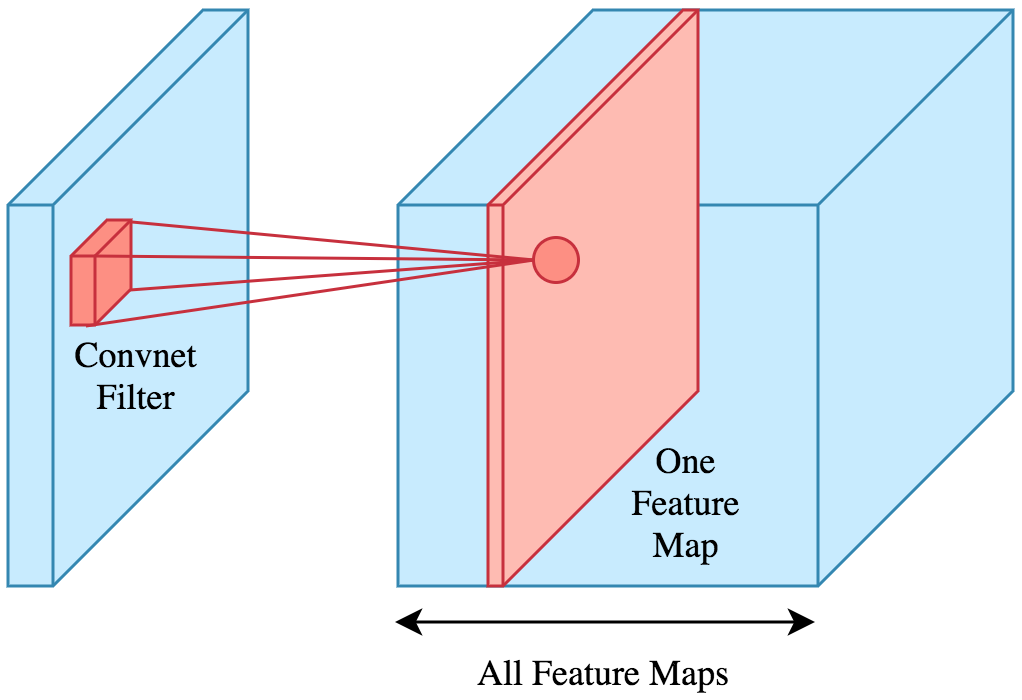
\includegraphics[width=0.5\textwidth]{pic_conv}
\end{figure}

In the simplest case, the trainable parameters of the network are only weights of a linear regression that optimized using gradient descent. Various techniques, such as batch normalization, dropout, or skip connections, are used to prevent overfitting or speed up the optimization of parameters.

In all the reviewed and proposed methods for 3D hand modeling, convolutional neural networks (CNNs) play an essential role.

\subsection{Blocks and cells}

In this section, we review two structures built from layers. Both of them mainly solve the problem of vanishing gradient. The first one is called residual block and was introduced as a solution for efficient training of deep networks with depth in hundreds of layers \cite{24} . Residual block returns not the output of the single final layer but the sum of multiple outputs. This design allows the optimizer to update weight at the beginning of the network more efficiently.

\begin{figure}
\caption{Residual learning: a building block \cite{24}.}
\centering
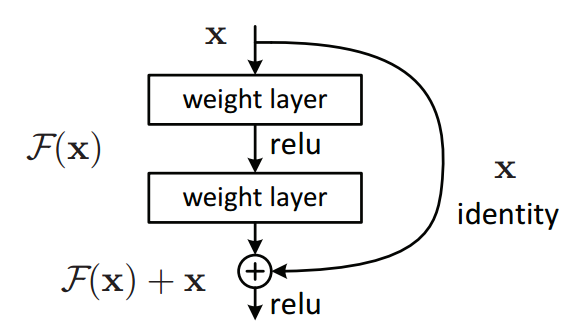
\includegraphics[width=0.5\textwidth]{res_block}
\end{figure}


The second structure is called LSTM cell and related to Recurrent Neural Networks that weren’t touched before in a thesis. RNNs are used for sequence modeling where there is a task of mapping one sequence to another. Each element of a sequence is fed to network cell, which extracts patterns of elements. The problem, in this case, again vanishing gradient for the case of long sequences and can be solved by LSTM cell. The sequence of computational operations is listed on equations 2.7-2.12 and illustrated on Fig 2.3.

\begin{figure}[h]
\caption{LSTM cell}
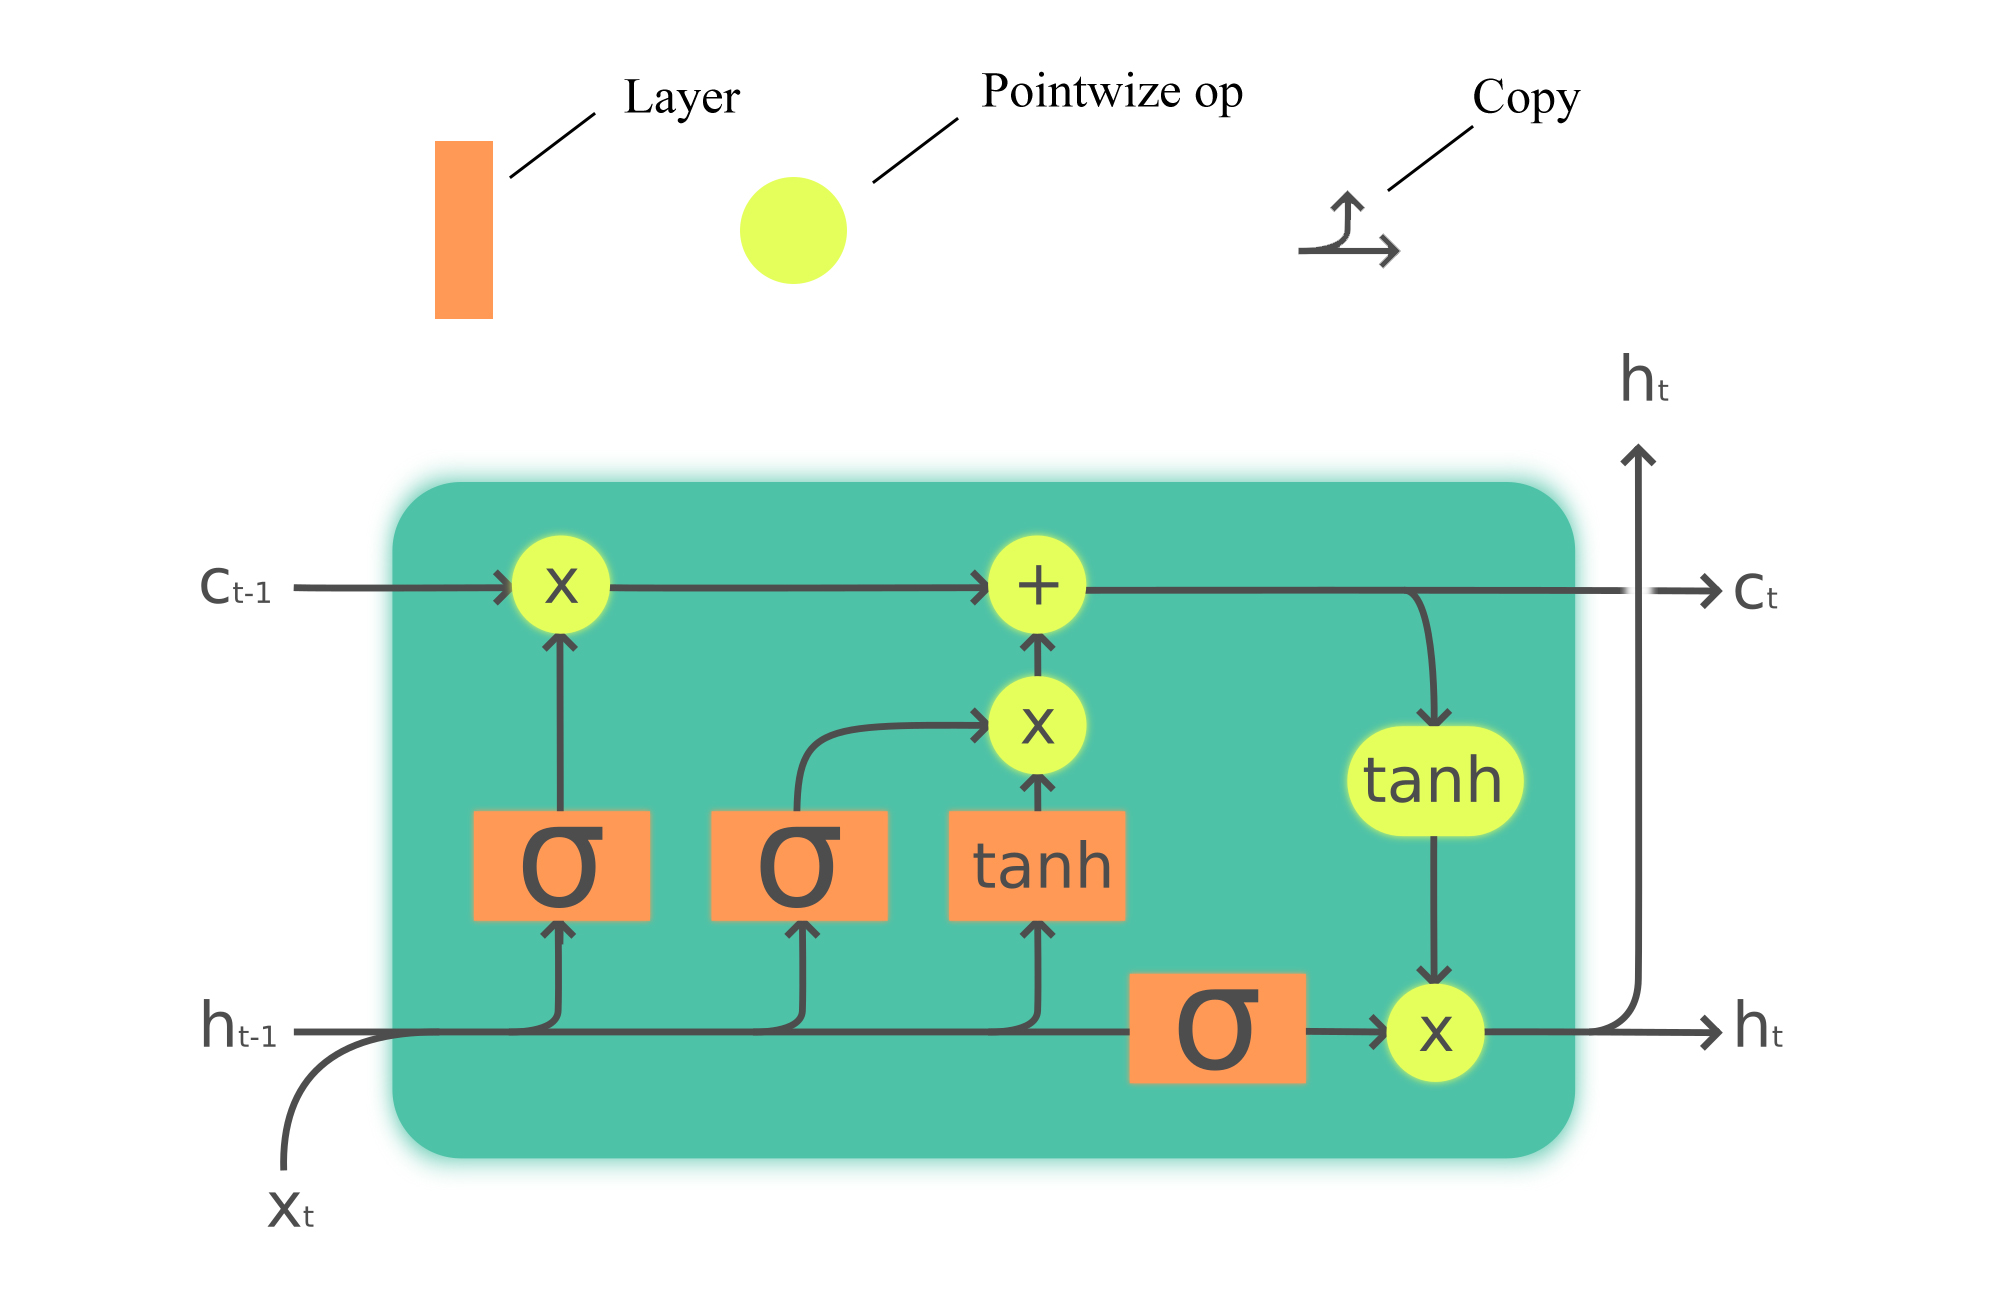
\includegraphics[width=1\textwidth]{lstm}
\end{figure}


\begin{equation}
f_t = \sigma_g(W_fx_t + U_fh_{t-1} + b_f)
\end{equation}


\begin{equation}
i_t = \sigma_g(W_ix_t + U_ih_{t-1} + b_i)
\end{equation}

\begin{equation}
o_t = \sigma_g(W_ox_t + U_oh_{t-1} + b_o)
\end{equation}

\begin{equation}
o_t = \sigma_g(W_ox_t + U_oh_{t-1} + b_o)
\end{equation}

\begin{equation}
c_t = f_t\circ c_{t-1} + i_t \circ \sigma_c(W_cx_t + U_ch_{t-1} + b_c)
\end{equation}

\begin{equation}
h_t = o_t\circ \sigma_h(c_t)
\end{equation}

\section{Methods for 3D shape estimation}

Most methods for 3D hand pose generation from a single RGB image can be generalized into four stages. The first stage is the detection of hands in the input image and cropping localized area; the second is the detection of hand key-points in 2D; the third is a mapping of 2D locations into 3D, and the fourth is a generation of the 3D hand model.


\begin{figure}[h]
\caption{Generalized schema of 3D hand pose estimation}
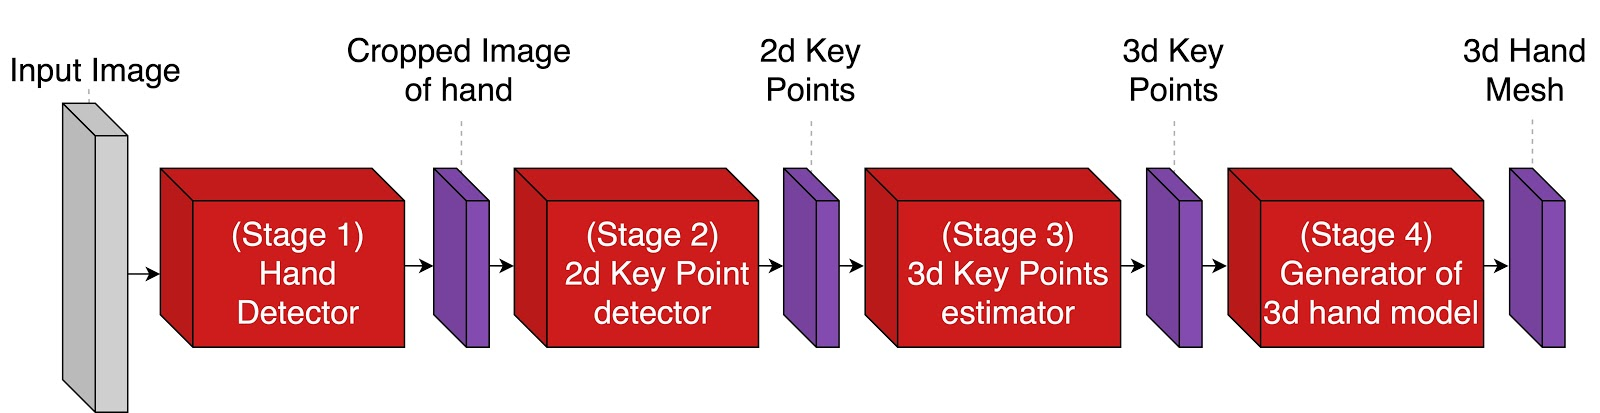
\includegraphics[width=1\textwidth]{schema3dr}
\end{figure}

\subsection{Networks for 2D key-point detection}
Estimation of 3D structures such as 3D key-points or 3D hand model is the hardest to train part of the pipeline. For higher accuracy of those stages, it is essential to accurately estimate 2D key-points of the hand, because this data contains two-thirds of the 3D locations. We will review a few models suitable to address tasks of 2D key-points estimation. We will discuss three CNNs, namely U-Net, Stacked Hourglass Network, and Open Pose. 

\begin{figure}
\caption{a) U\-Net architecture \cite{25} , b) Stacked Hourglass Network \cite{27}}
\centering
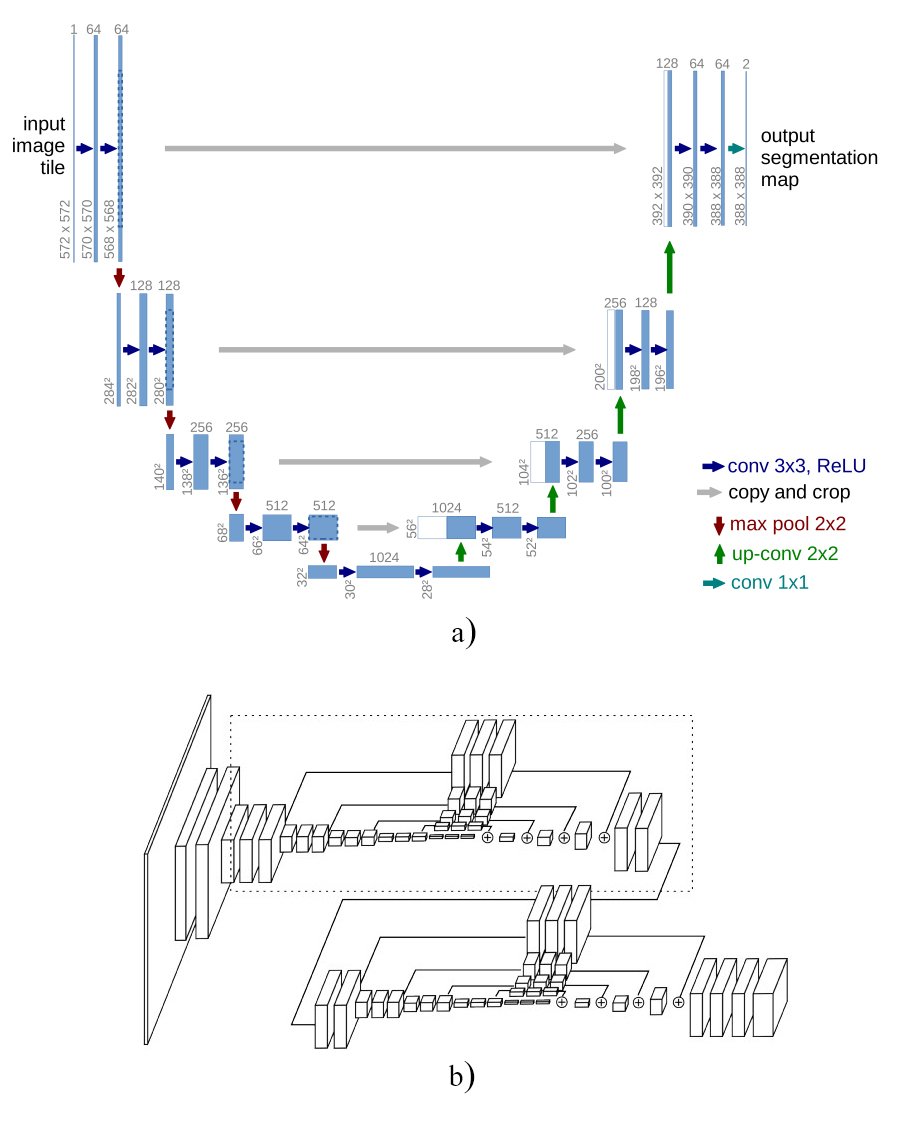
\includegraphics[width=0.7\textwidth]{nuets}
\end{figure}

The U\-Net is an architecture which first extracts image features by downsampling layers and then upsamples them alongside sequential concatenation of outputs from previous layers \cite{25}. U-Net like architectures have proven to work with the task of 2D key-points detection \cite{26}.

Stacked Hourglass Network extends the idea of U-Net and stacks several architectures of a similar type into one pipeline with supervision after each step \cite{27}. Building blocks are residual and skip connections are implemented by the addition of feature maps rather than concatenation.

Open pose detector is a CNN that consists of multiple computational stages and two parallel computational pipelines. Each stage is estimating both locations of 2D key-points and connections between them. All stages except the first one are estimating information about joints based on previous results. In such a way, the detector is reffing computational results with each iteration.

\subsection{Systems for 3D reconstruction}

The paper \cite{10} introduces a three-stage algorithm that localizes the hands and determines the key-points in 2D at the first two stages and calculates 3D reconstruction at the third is studied in the paper. 

\begin{figure}
\caption{Illustration of parallel computational pipelines used in Open Pose \cite{PCP}}
\centering
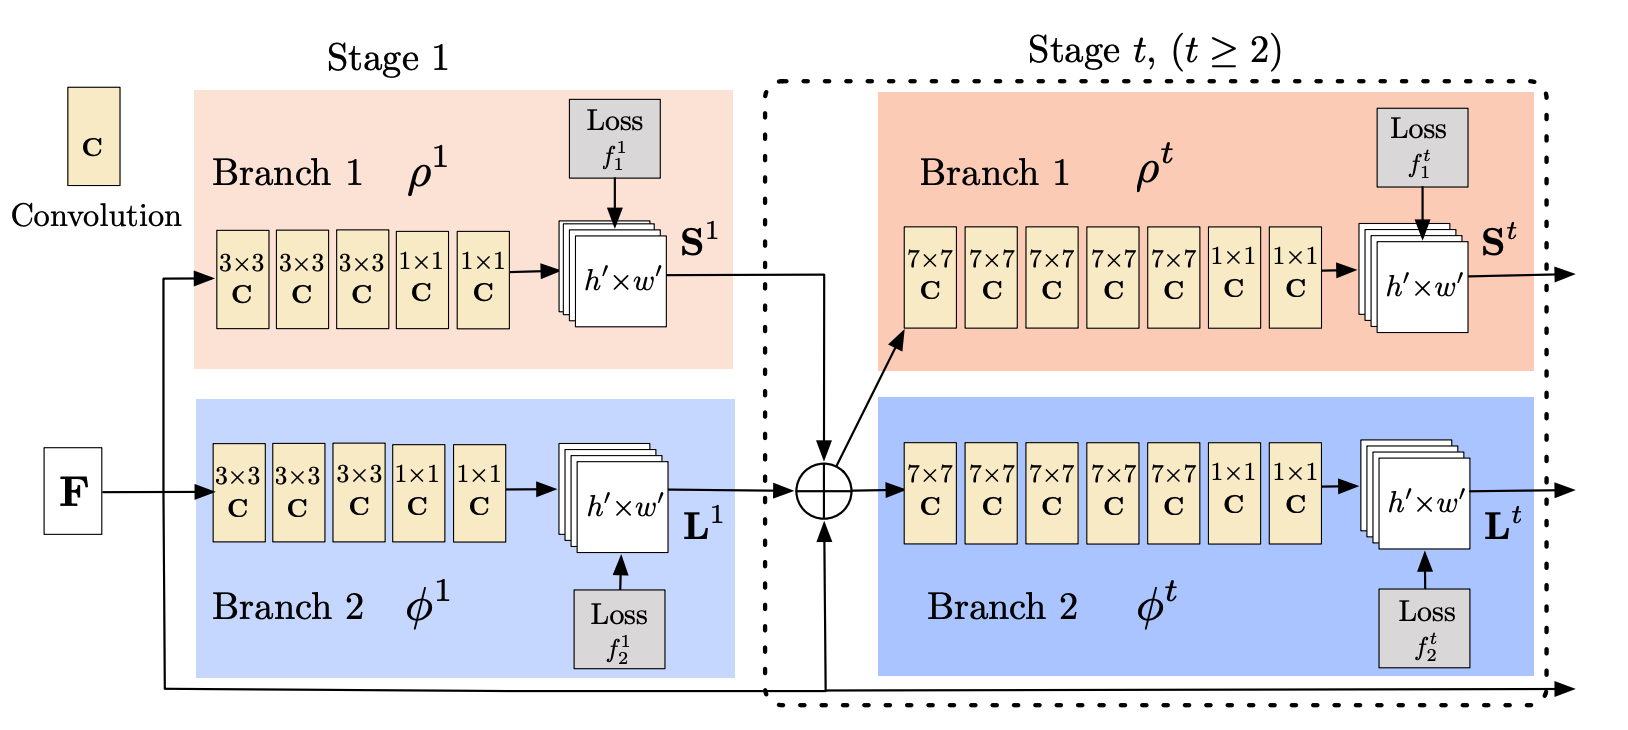
\includegraphics[width=1\textwidth]{methodPCP}
\end{figure}


The first stage is the YOLOv2 neural network (‘you only look once’), which identifies the position of the hands. YOLOv2 is a CNN which used for localization and classification of multiple objects at once.

The localized hands are passed to the OpenPose detector.

These two neural networks localize 21 2D key-points on the video frames, which are then used as a target in the inverse kinematic optimization problem. A distinct drawback of this method is the limitation caused by the error of the OpenPose detector. This error causes the algorithm to optimize 3D locations using the wrong 2D key-points. Nevertheless, the addition of a hand position from a different view makes it possible to improve the optimization problem, and hence the accuracy. The runtime of the method on Nvidia GTX 1070 GPU is close to 53 ms. 

The work \cite{23} describes one of the few methods which fully reconstructs the 3D shape of the hand. It introduces a graph convolutional neural network (CNN) for generating 3D mesh. The work uses centered images of hands as input, thus hand detection was not necessary. Therefore, the first part of the approach is 2D key-point detection, which is based on Stacked Hourglass Networks. The second is the encoding of 2D features, and the third is 3D reconstruction with a graph CNN network. The network outperforms state-of-the-art methods on RHD \cite{13} and STB \cite{14} datasets. The runtime of the method on Nvidia GTX 1080 GPU is, on average, 19.9ms. The pretrained model is available, but the training dataset is not.

\begin{figure}
\caption{Scheme of the method described in paper 3D Hand Shape and Pose Estimation from a Single RGB Image. \cite{23}}
\centering
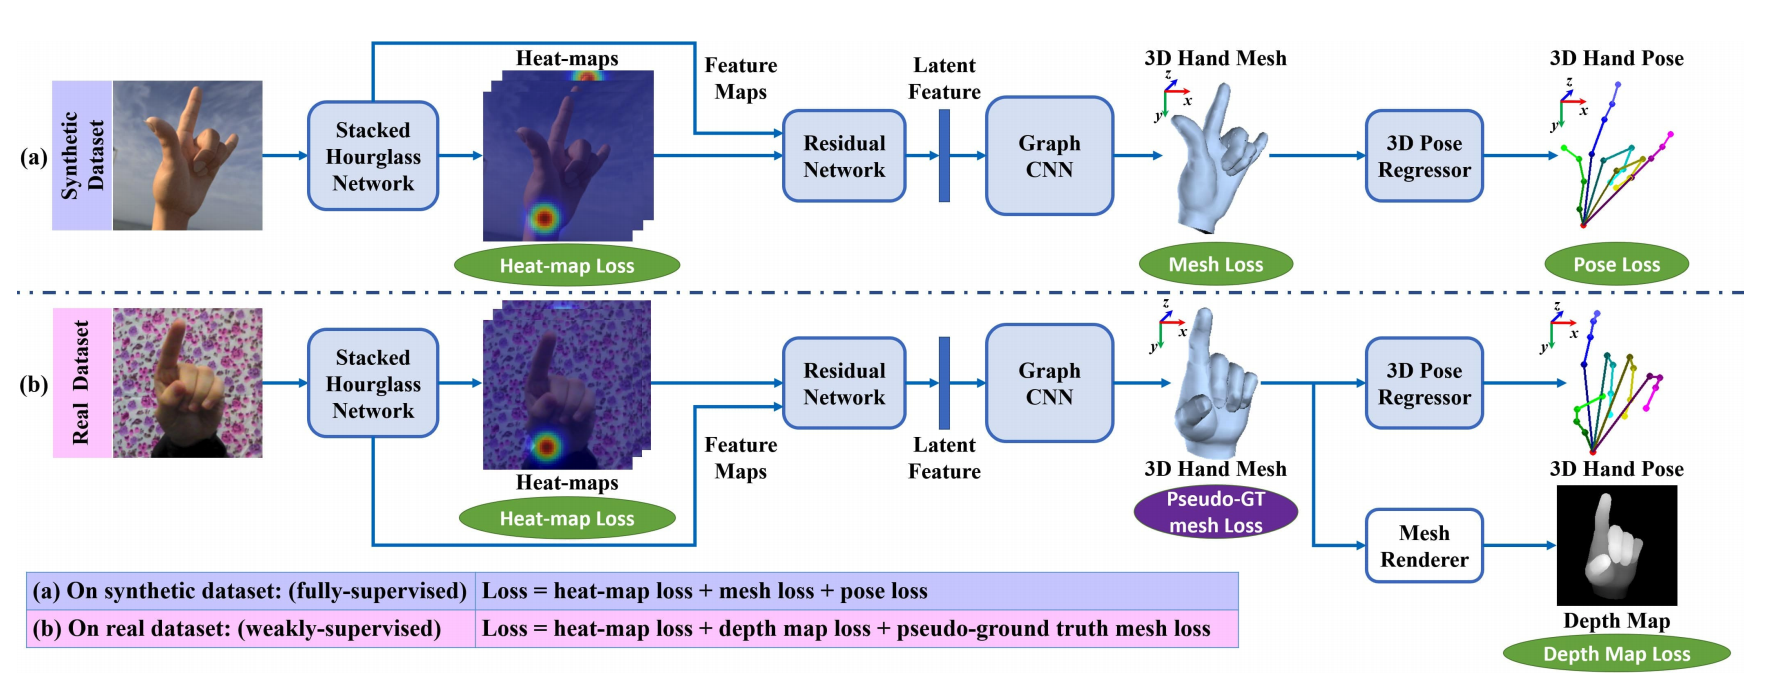
\includegraphics[width=1\textwidth]{method2}
\end{figure}

\subsection{MANO model}

MANO is a differentiable parametric model of the hand, which can be integrated into computational pipelines. MANO learned from around 1000 3D scans of hands in various poses. The model takes as input parameters of pose and shape, which then mapped to the cloud of points, which represent the hand surface \cite{MANO:SIGGRAPHASIA:2017}. 
\setcounter{mtc}{2}
\chapter{3D hand pose reconstruction}

\section{Overview of proposed methods}

The work is aimed at solving three tasks: studying the influence of preliminary frames on the reconstruction of video sequences; investigating the process of results refinement; image reconstruction of hands displaying the letters of American Sign Language. We are solving all by the introduced 3-stage computational pipeline, where every stage is a neural network designed to solve a small task.

The proposed method can be described by the schema of 3D hand pose estimation close to specified in Fig 2.4. Except it does not have the first stage of the hand localization stage and work directly with centered hands. In that way, the introduced method can be generalized to the sequence of architectures A, B, and C. We sequentially compute locations of 2D key-points by network A, depth for each key point by B, and after that, calculate the vector of MANO parameters from key points by C. 

In total, 13 ANN architectures were tested for tasks A, B, and C combined. Six designs were studied as candidates for network A, five - for B, and two for C. The networks A and B can be considered as one architecture for 3D key-point detection. For A and B, we were focused on the influence of two factors on the training process. Those factors are additional frames at input and refinement of predictions. To investigate the difference in the training trends was developed a system for parallel training and evaluation of multiple networks. Network C stands alone from networks A and B because it doesn't process images. Its task is to estimate the vector of MANO hand surface generation parameters from a set of 3D points. This stage finishes the computational pipeline, which allows us to annotate a subset of American Sign Language.

\section{Neural networks for 2D key point detection}

Network A takes as an input RGB information and outputs 22 heatmaps of size 224x224, \{H1, H2,..., H2\}, where each heatmap Hk from indicates the probability of observing the kth keypoint and for k=22 probability of no key points. A similar approach has proven to work efficiently in \cite{PCP}.

\begin{figure}
\caption{Building blocks and assembled networks for 2D key point detection: a)U-Net architecture; b)Hourglass Like Module c)Architecture of STH\_2; d)Architecture of STH\_3.}
\centering
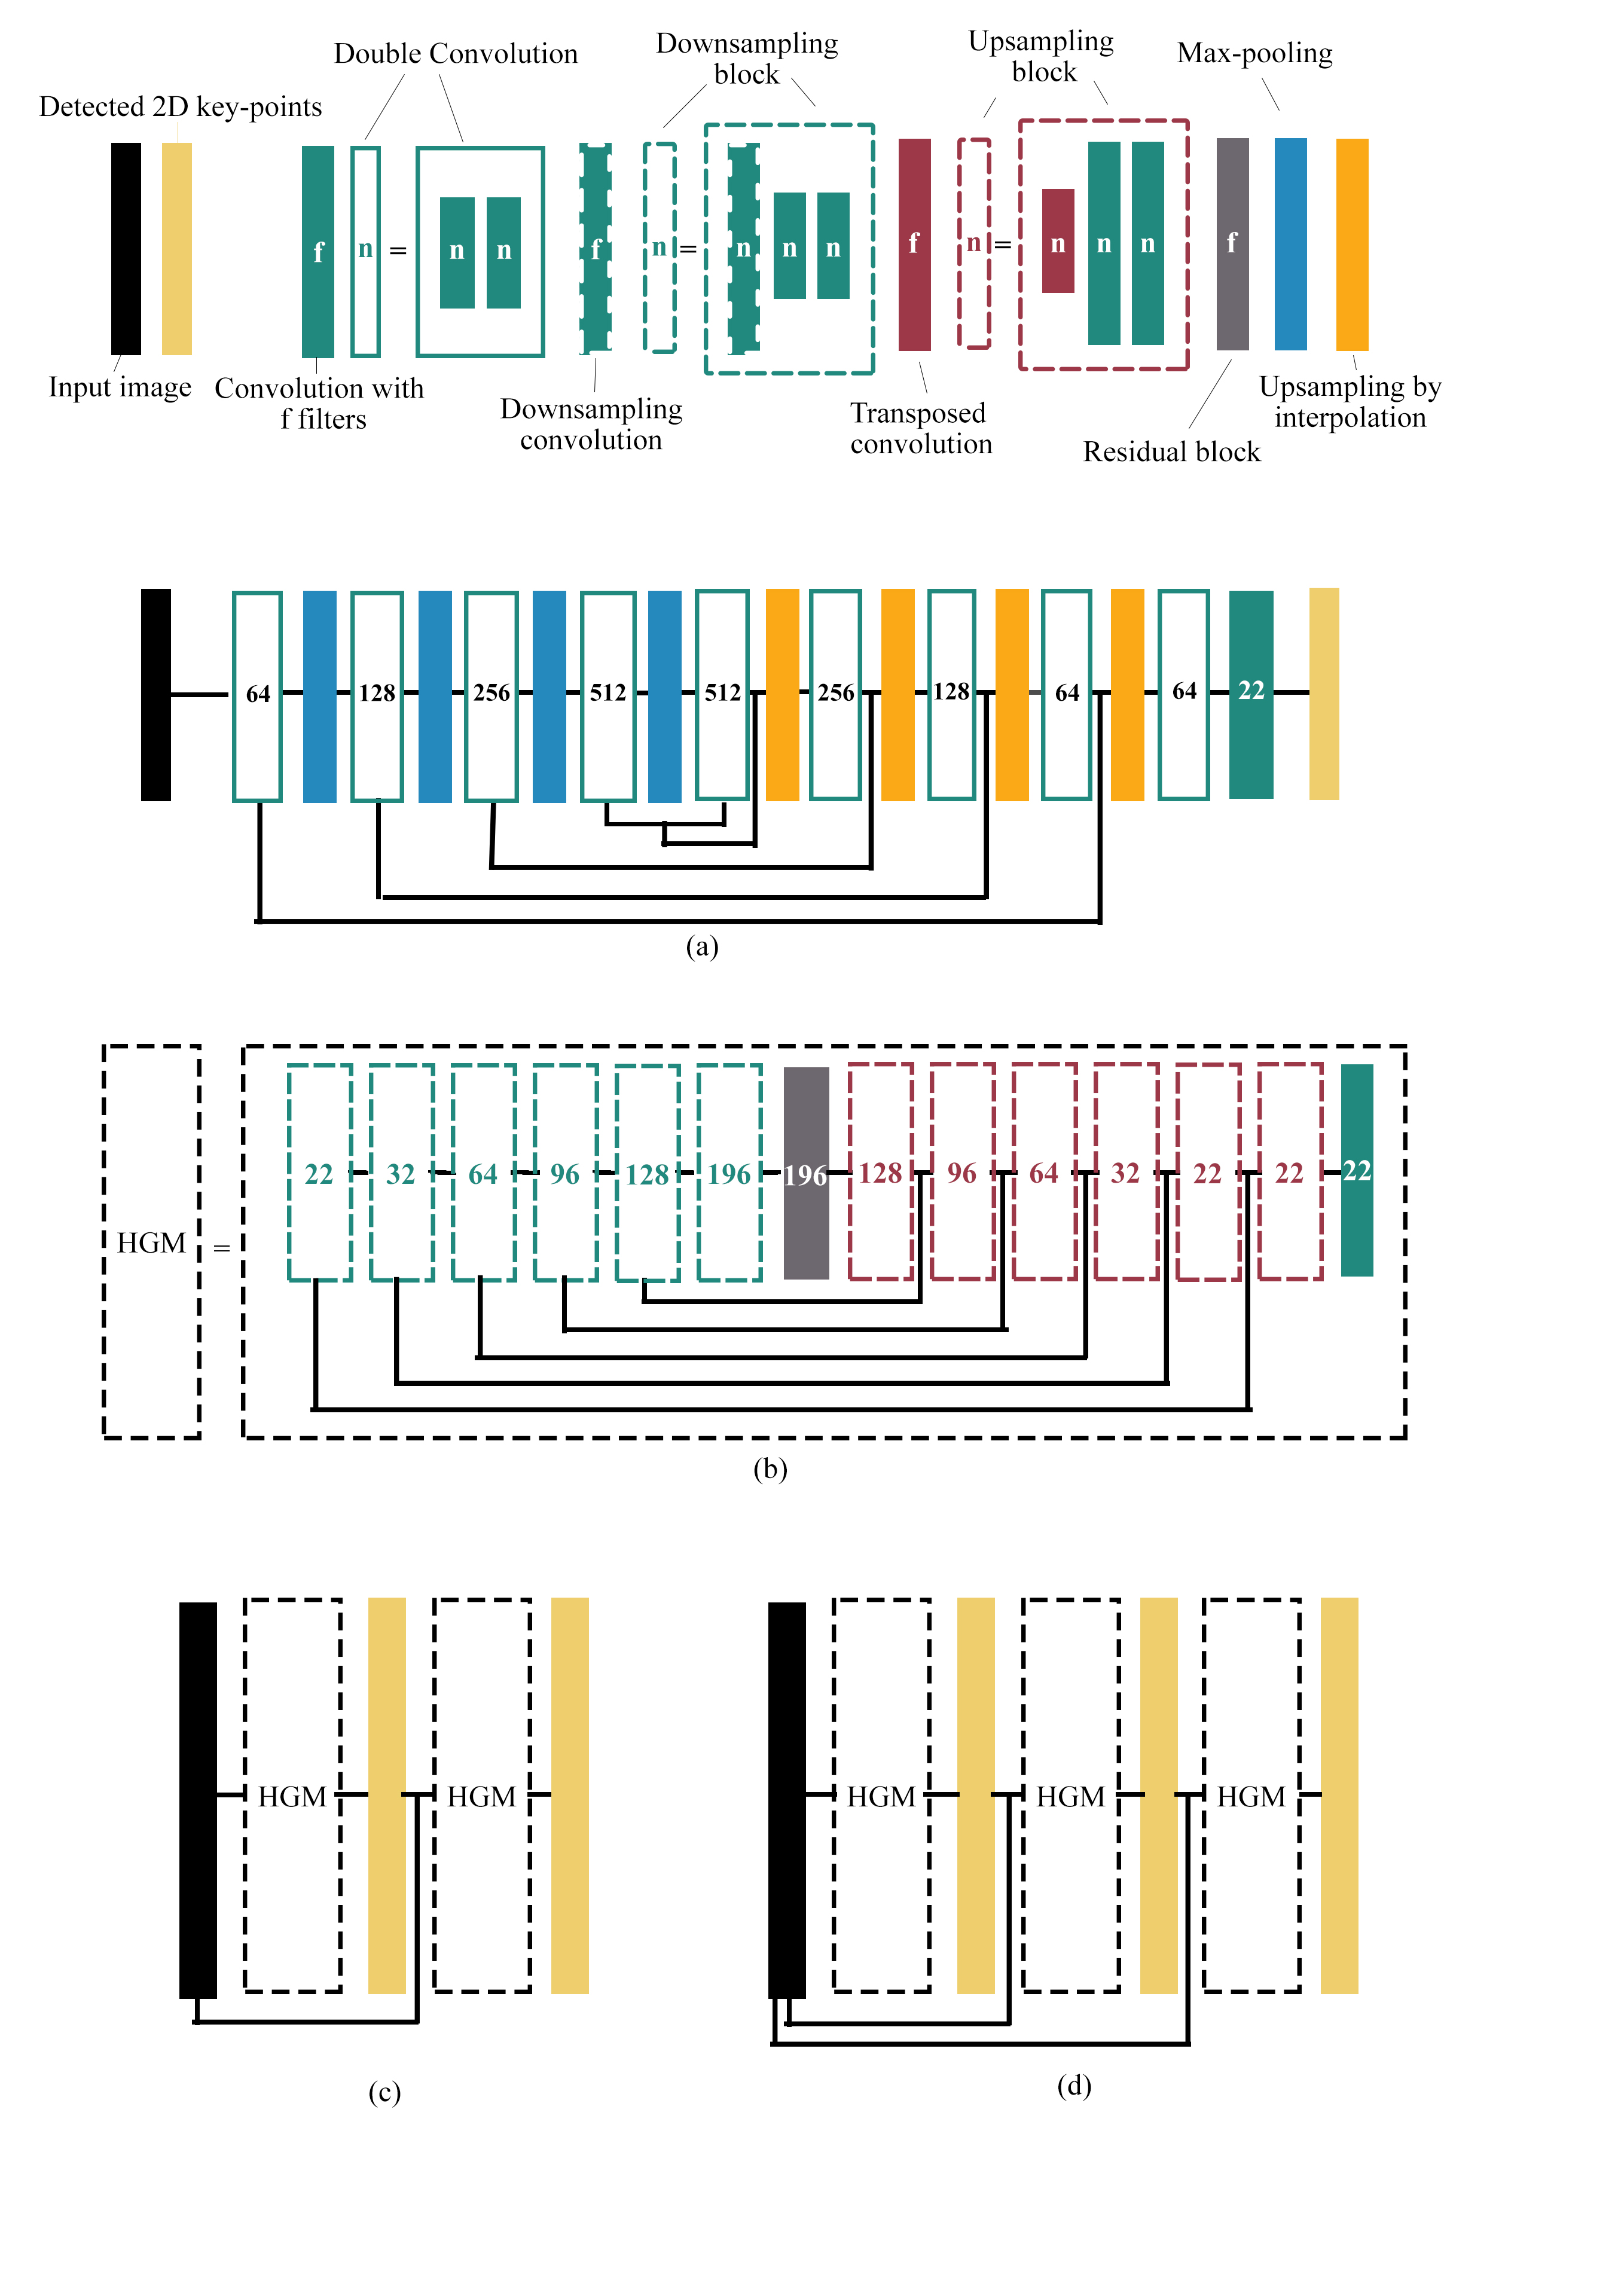
\includegraphics[width=1\textwidth]{finala}
\end{figure}

Two Stacked Hourglass Like and one U-Net architecture are candidates for main network at stage A for 2D key-point detection. Each candidate has a variation for video and image processing. In total, there are 6 architectures for 2D key point localizations with the following id’s: UNET\_VID, STH\_2\_VID, STH\_3\_VID, UNET\_PIC, STH\_2\_PIC, STH\_3\_PIC. Where ‘STH\_’ stands for Stacked Hourglass like architecture; \_VID means that input contains concatenated RGB frames and 2D points of the previous frame;  \_PIC means that input contains a single RGB image.

Let kc denote the convolutional layer with k filters and stride 1, kd - the convolutional layer with k filters and stride 2, ku - the transposed convolutional layer with k filters and stride 2, kfc - fully connected layer with k neurons, mp - max pooling with 2x2 filter, up2 is x2 upsampling by interpolation, kr - residual block from Fig 2.2 with k filters. All convolutional layers except for the last one are followed by batch normalization and ReLU activation.

Implementation of U-Net is: 64c, 64c, mp, 128c, 128c, mp, 256c, 256c, mp, 512c, 512c, mp, 512c, 512c, up2, 256c, 256c, up2, 128c, 128c , up2, 128c, 128c, up2, 64c, 64c, up2, 64c, 64c, 22c. Outputs of layers are concatenated in order shown in Fig. 3.1 a).

The architecture of proposed HGM is: 22d, 22c, 22c, 32d, 32c, 32c, 64d, 64c, 64c, 128d, 128c, 128c, 196d, 196c, 196c, 196r, 128u, 128c, 128c, 96u, 96c, 96c, 64u, 64c, 64c, 32u, 32c, 32c, 22u, 22c, 22c, 22u, 22c, 22c, 22c. Outputs of layers summed in order shown in Fig. 3.1 b). 

The architecture of STH\_2 consist of two hourglass modules where the second module takes as input image concatenated with the initial prediction from the first module, as illustrated in Fig 3.1 c). The architecture of STH\_3 set in the same way as STH\_2, except there is one additional module for refinement, as shown in Fig 3.1 d).

It is important to accentuate that architectures drastically differ in size. 

\begin{table}[H]
\small
\begin{tabularx}{1\textwidth}{sbbb}
 \hline
 net\_id & num\_of\_parameters & num\_of\_refinements & skip-connection type \\
 \hline
STH\_2\_PIC &
6106056 &
2 &
addition
\\
\hline
STH\_2\_VID &
6115956 &
2 &
addition 
\\
\hline
STH\_3\_PIC &
9161262 &
3 &
addition 
\\
\hline
STH\_3\_VID &
9176112 &
3 &
addition 
\\
\hline
UNET\_PIC &
13396694 &
1 &
concatenation
\\
\hline
UNET\_VID &
13411094  &
1 &
concatenation
\\
\hline
\end{tabularx}
\caption{\label{tab:res_0}Differences between nets A}
\end{table}


\section{ANN for depth estimation (Network B)}

Network B is used for the estimation of 21 depth values for each key point. We propose 5 architectures for depth estimation marked as B\_PIC, B\_VID, B\_R\_PIC, B\_R\_VID, AB\_PIC. Where B\_R means that output is calculated multiple times (refined), AB stand for additional usage of features from network A, \_VID means that input contains concatenated RGB frames and 2D points from current and previous frame, as well as depth from the previous frame;  \_PIC means that input contains concatenated RGB data with 2D key points from a single image. 

\begin{figure}
\caption{Studied building blocks and networks for depth estimation: a)Feature Extractor; b)Dense layers with additional depth inputs; c)Dense layers with additional depth outputs.}
\centering
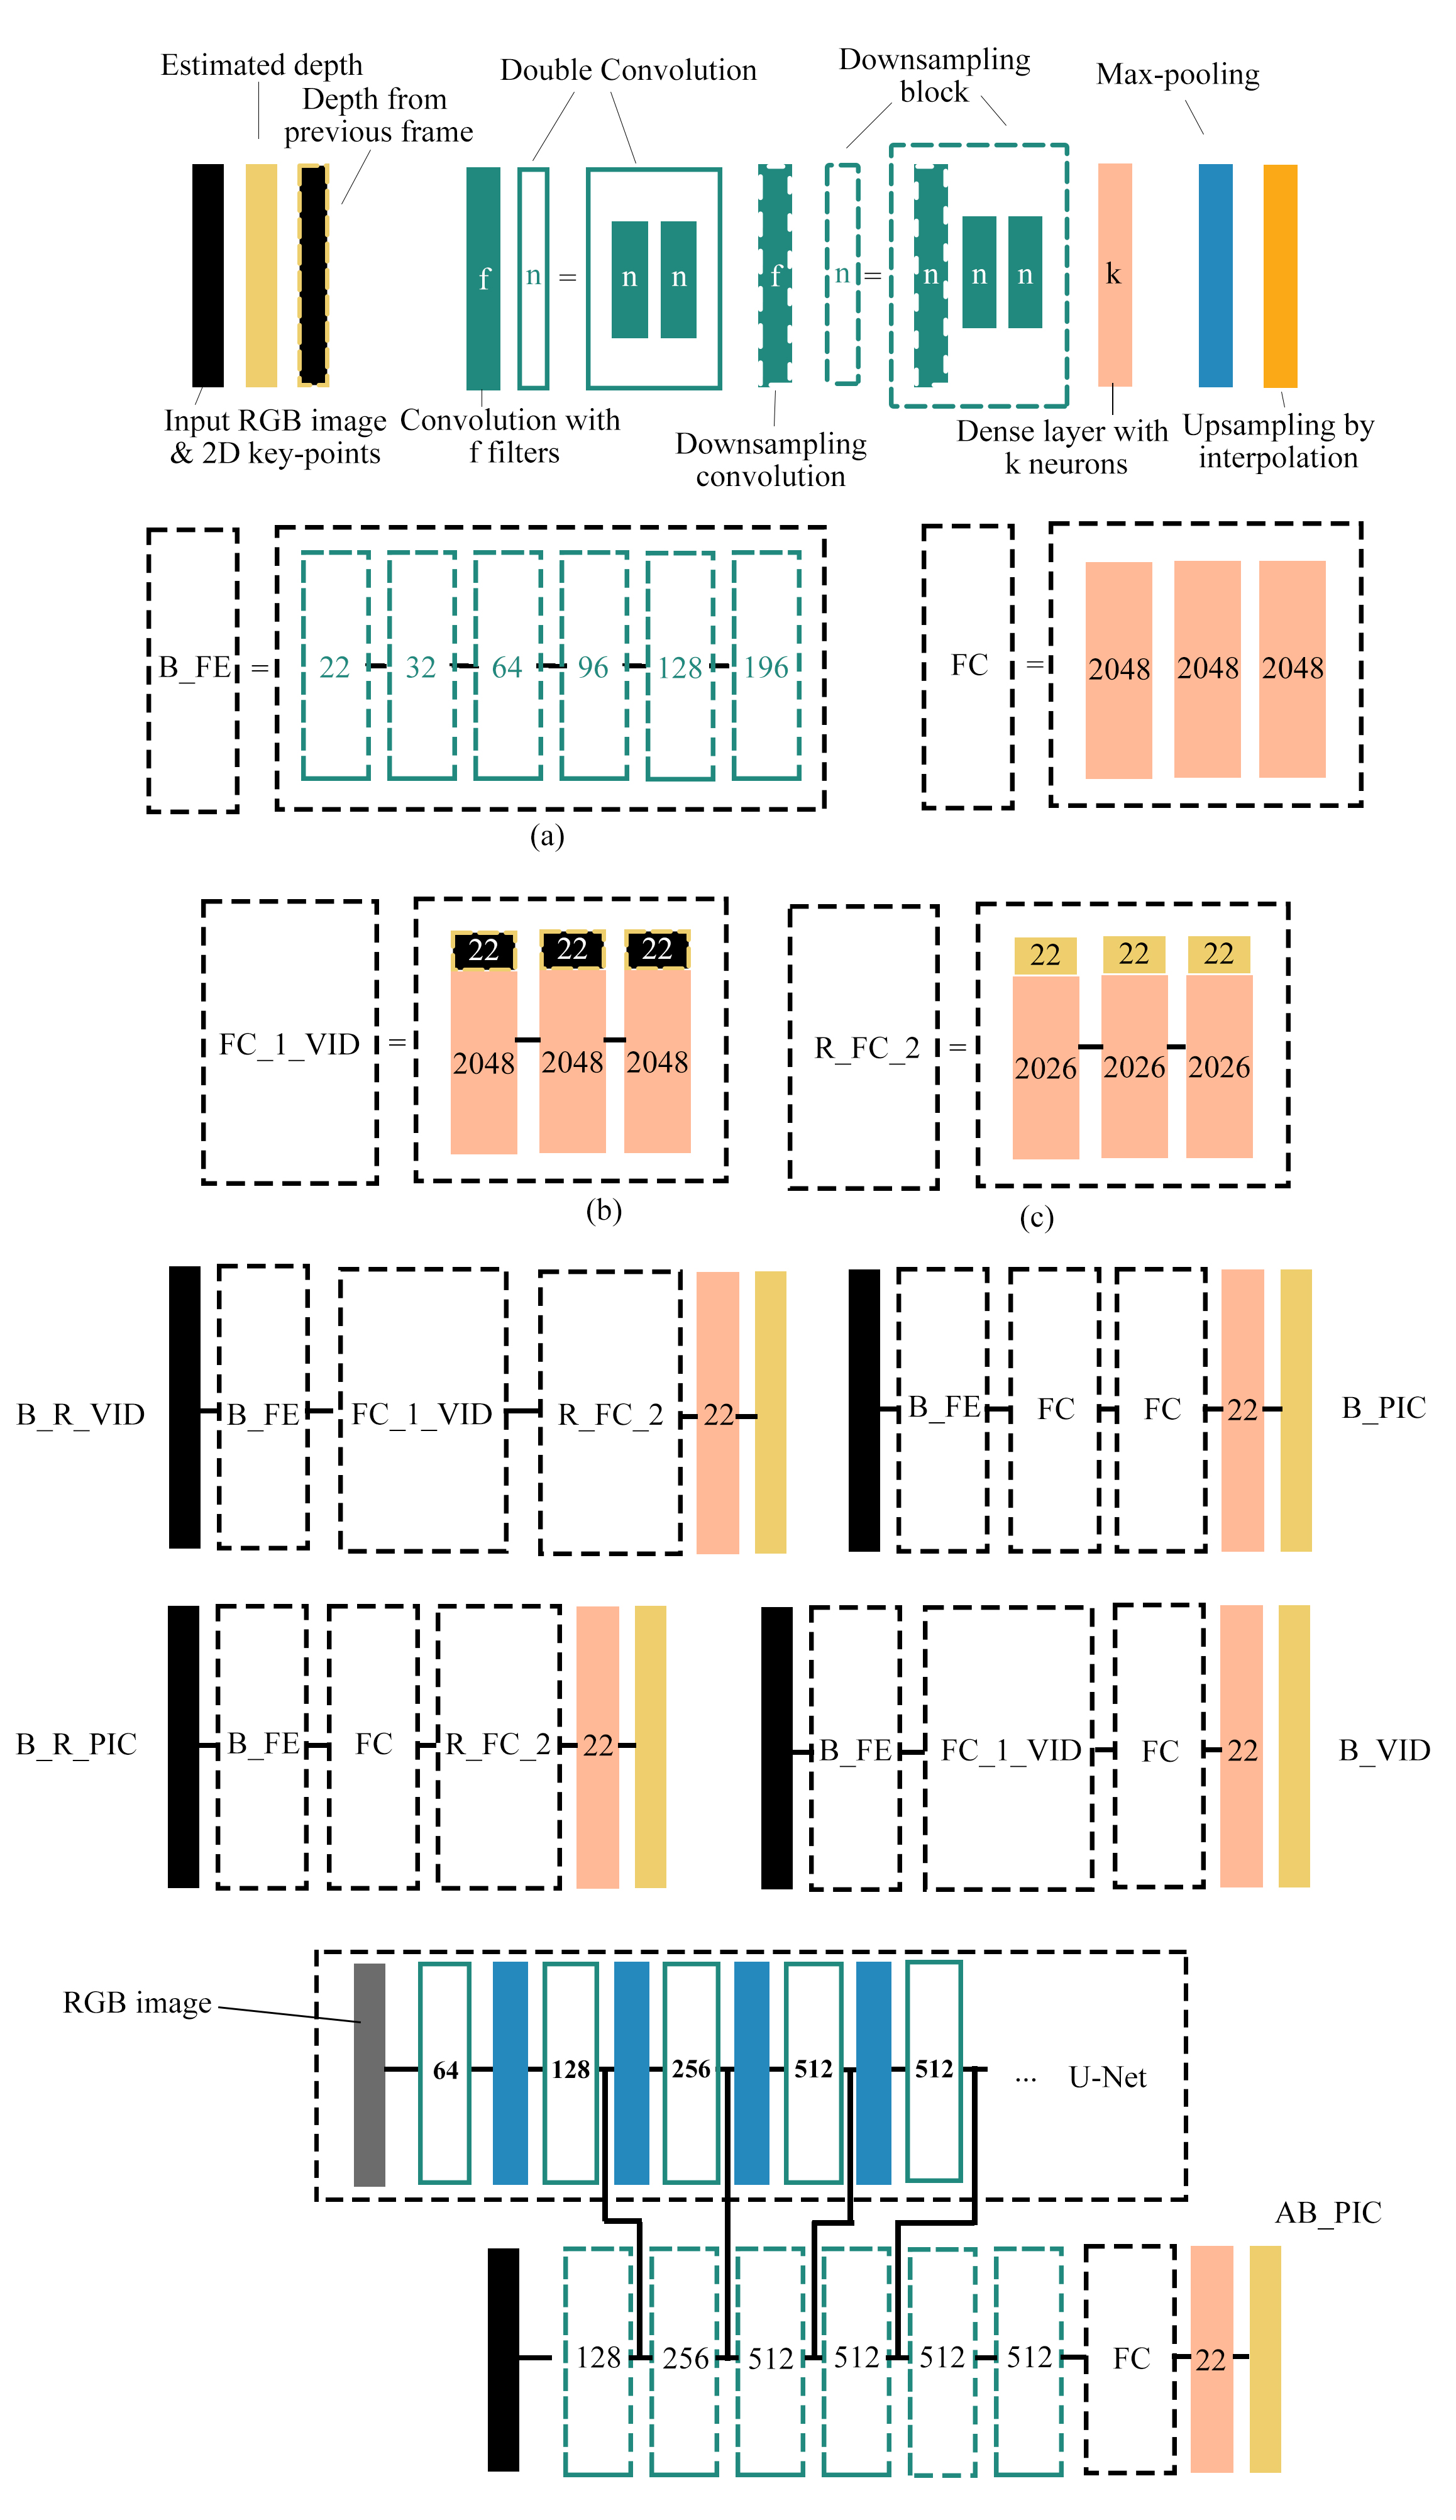
\includegraphics[width=1\textwidth]{finalb}
\end{figure}

All networks have two parts. The first part is Feature Extractor (FE), and the second is a set of fully connected blocks (FC). The set of convolutional layers followed by dense layers is an effective solution for the image to vector problems \cite{m2}. Architecture of FE is same for B\_PIC, B\_VID, B\_R\_PIC, B\_R\_VID: 16d, 16c, 16c, 32d, 32c, 32c, 64d, 64c, 64c, 128d, 128c, 128c. Feature Extractor of network with id AB\_PIC has following architecture: 128d, 128c, 128c, 256d, 256c, 256c, 512d, 512c, 512c, 512d, 512c, 512c, 512d, 512c, 512c, 512d, 512c, 512c. Outputs of Feature Extractor layers for network AB\_PIC concatenated with outputs of UNET layers in a way shown at Fig. 3.2
    

Sets of fully connected blocks are different for all networks. Networks B\_PIC, B\_VID, B\_R\_PIC, B\_R\_VID ends with 7 dense layers. Networks that work with video sequences have additional inputs at first three blocks, as shown at pic 3 b). Id's of networks with refinement of results marked with \_R and optimized so that each of 4 ending layers has 22 neurons responsible for depth info. Network AB\_PIC has 4 fully connected layers with no additional info or refinement, and the output of the last layer only is depth.

\section{Network for estimation of shape parameters}

The 3D shape of a hand is represented as a mesh with 778 vertices. Those vertices are encoded in 51 parameters and decoded by the MANO model. We convert 21 3D key-points into MANO parameters by network C.
    
\begin{figure}[h]
\caption{Studied architectures for shape parameterization. a) Shema of MANO input-output mapping; b)Architecture of C\_RNN network; c)Architecture of C\_MLP network.}
\centering
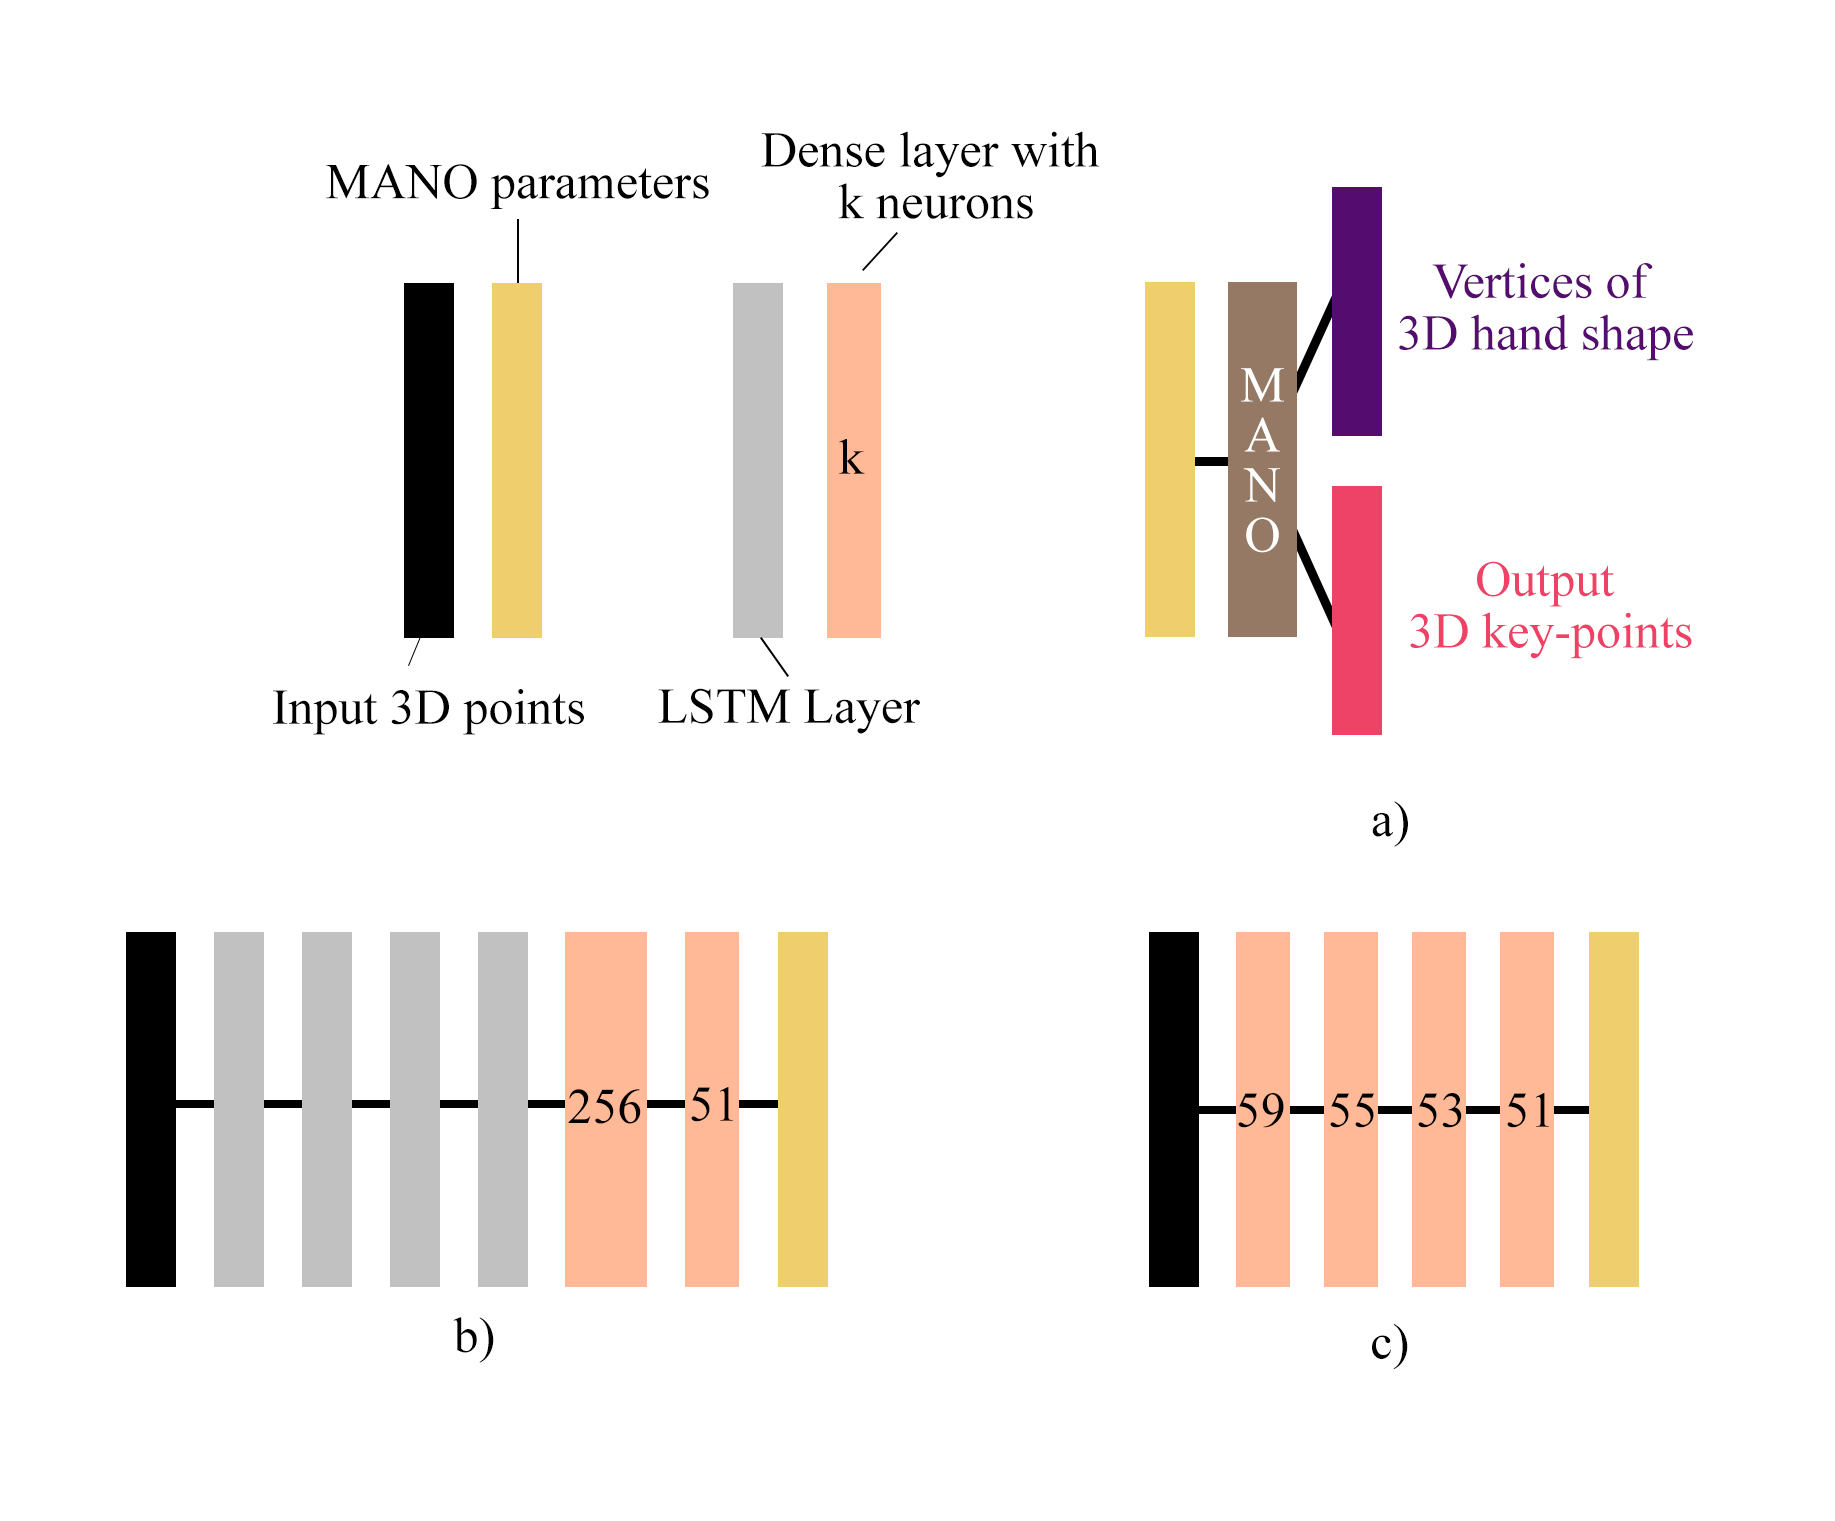
\includegraphics[width=0.6\textwidth]{finalc}
\end{figure}


We considered two architectures as candidates for network C. The first model has id 'C\_RNN' and consists of 4 LSTM layers and fully connected output. The second model with id 'C\_MLP' is a set of fully connected layers. Illustrated in Fig. 3.3.
 




\setcounter{mtc}{3} 
\chapter{Experiments and results}

\section{Datasets}

Several datasets were examined, and the most suitable was selected for our task. Large portion of datasets for 3D reconstruction contain depth maps, key points, but not RGB image: NYU, ICVL, MSRA15, BigHand2.2M, SynHand5M, FHAD, MSRC\(FingerPaint\), HandNet, Hands in Action, MSRA14 \cite{1,2,3,4,15,16,17,18,19,20}. For the problem of reconstruction from a single image, most appropriate datasets are those that feature both RGB records and key points: FreiHAND, GANerated Hands, EgoDexter, SynthHands, STB, Dexter+Object, UCI-EGO, MHP \cite{4, 11, 12, 14, 21, 22}. The possible complication of combining different datasets is that the number of key points, record types, and camera parameters may not match. We left only datasets with a central position of a hand and 21 labeled key points.

FreiHAND Dataset is a hand pose dataset for hand pose estimation from a single image. The dataset contains shots with 4 different data augmentations annotated with 21 key points for 2D and 3D spaces. The total amount of training samples is 130240 for single view training. So 32560 poses for training \cite{4}. 

GANerated Hands Dataset contains 330,000 examples annotated with 21 key points for 2D and 3D spaces. The downside of this dataset is that images are synthetically generated and have distorted edges of hands. All of them are recorded from one viewpoint \cite{11}.

SynthHands is a synthetic dataset, which provides information about 63,530 frames recorded from 5 views. Learning examples contain both RGB and depth records and represent records with and without object interaction. Data annotated for 21 points in 3D space. Hands were generated using Unity3D engine but animated using data captured from real motion \cite{12}. 

We chose FreiHAND Dataset and SynthHands dataset for training and evaluation, respectively. Also, we used Home Object Dataset for background augmentation of SynthHands dataset. Home Object Dataset \cite{HOD} contains 450 photos of random objects. Augmented SynthHand dataset denoted in work as 'SynthHands\_A'.

\begin{table}
\begin{tabularx}{1\textwidth} { 
  | >{\raggedright\arraybackslash}X 
  | >{\centering\arraybackslash}X 
  | >{\centering\arraybackslash}X 
  | >{\raggedleft\arraybackslash}X | }
 \hline
 Dataset name & Number of images & Synthetic / Real  & Number of camera views \\
 \hline
 FreiHAND  & 32,560  & Real  & 1 \\
 \hline
 GANerated Hands  & 330,000  & Synthetic  & 1 \\
 \hline
 SynthHands  & 63,530  & Synthetic  & 5 \\
\hline
\end{tabularx}
\caption{\label{tab:table-name}Datasets info}
\end{table}

Besides annotated datasets for training and testing, we used the ASL dataset for reconstructions. Kaggle ASL dataset \cite{ASL} contains 87000 of hand poses. Images were labeled for the task of sign language recognition. There are 26 classes for letters and three classes with images for SPACE, DELETE, and NOTHING.

\section{Data preprocessing algorithms}

As there were no 3D annotated video dictionaries of sign language available at the time of the study, an artificial sequencing procedure was proposed. It is proposed to sort images of hands with annotations to mimic real-world transition of hands from frame to frame. For each record in a dataset, we search one with the closest 3D position and use both in the training process. Because frame n and n-1 have close 3D positions in the real world, such sorting allows us to use a non-video dataset for usage in tasks of video processing. Usage of fake video sequences different from real-world applications in two ways. First - the transition between hands not as smooth as in the real world. Second - in our study, we used ground truth annotation for the previous frame at the input for the network. Because the previous frame is more random than in real videos - ground truth data in a way mimic noisy prediction for the previous frame. But, of course, training on annotated synthetic video does not suffer from an accumulation of noise as much as if for each next frame, we would use the previous prediction of the network.

To solve the task of shape reconstruction, we are adding additional data preprocessing. First, we are masking density estimation of MANO annotations to sample more data. We are creating a new dataset by sampling vectors from distribution, passing it to a MANO model, and obtain corresponding 3D shape and key-points. The new dataset allows us to train network C on a large number of sampled vectors. 

\section{Training 3D shape estimation stages}

For training and testing was used Frei Hand Dataset split for test and train subsets in ratio 1:4. As an additional dataset for evaluation, we used SynthHand dataset with and without the addition of background.

It is needed to account for different scales of key point spaces. Datasets or hand models encode certain magnitude of hand, so simultaneous work with different coordinates requires unification. In our case MANO model, Synth Hand Dataset and Frei Hand Dataset are all in different scales. Frei Hand Dataset hands are ~990 times smaller than MANO reconstructions. In contrast, Synth Hand Dataset is ~0.94 times smaller than MANO hands. It does not influence training for 2D key-points because data projected to the image plane and unified in that way. For depth, it is more important to have annotation in one scale. Networks for depth estimation learn both ratios between fingers depth as well as absolute depth. We have transformed the absolute depth of SynthHand Dataset annotations to match the average depth of FreiHand Dataset. For calculation of 3D error, we transformed all coordinates to MANO model space. It is the shortest way to achieve unification given that vector of MANO parameters is part of our pipeline, and that scale is used for training.

% ###################################################################################################################################
\subsection{Training and testing of networks for 2D key-point detection} 

We trained and tested 6 architectures in parallel. Adam optimizer was used with learning rate 0.0001 and trained on mini-batches of size 4 from FreiHand dataset for 40820 steps. We tested Mean Squared Error of predicted probabilities of location for each key point as well as absolute distance between the predicted location of key point and ground truth in 2D. For each network, we tested performance on 300 random images from 4 datasets. Results of testing on the train and test subsets of FreiHand Dataset are presented in tables 4.4 and 4.5, respectively. Metrics measured on Synth Hand Dataset presented in Table 4.6 for data without background, and table 4.7 tests on images with augmented backgrounds.

Results in tables 4.2-4.5 show that providing additional video frames decreases mean errors in most cases by 5-30\%. And additional refinement improves results only after a certain number of iteration. The proposed variation of Stack Hourglass Model has better results than larger UNET architecture on train subset as well on Synth Hand data-set with and without background. But since it has a larger error on test subset on real data, we assume that UNET generalizes better.

\begin{table}[H]
\small
\begin{tabularx}{1\textwidth}{sbbbbbb}
 \hline
 & STH\_2\_PIC & STH\_2\_VID & STH\_3\_PIC & STH\_3\_VID & UNET\_PIC & UNET\_VID \\
 \hline
mse \\
(points) &
2.64E+02 &
1.63E+02 &
1.92E+02 &
1.67E+02 &
2.15E+02 &
1.16E+02 
\\
\hline
l1 \\
(points)&
10.097 &
7.198 &
7.861 &
7.545 &
7.192 &
6.259 
\\
\hline
mse \\
(heatmaps) &
8.11E-04 &
7.68E-04 &
7.89E-04 &
7.82E-04 &
7.60E-04 &
7.62E-04 
\\
\hline
\end{tabularx}
\caption{\label{tab:res_1}Mean errors on train dataset for networks A}
\end{table}

\begin{table}[H]
\small
\begin{tabularx}{1\textwidth}{sbbbbbb}
 \hline
 & STH\_2\_PIC & STH\_2\_VID & STH\_3\_PIC & STH\_3\_VID & UNET\_PIC & UNET\_VID \\
 \hline
mse \\
(points)&
2.86E+02 &
2.01E+02 &
2.17E+02 &
1.89E+02 &
1.92E+02 &
1.67E+02 
\\
\hline
l1 \\
(points)&
10.582 &
8.448 &
8.507 &
8.59 &
6.906 &
7.757 
\\
\hline
mse \\
(heatmaps) &
8.26E-04 &
8.11E-04 &
8.09E-04 &
8.24E-04 &
7.77E-04 &
7.99E-04 
\\
\hline
\end{tabularx}
\caption{\label{tab:res_2}Mean errors on test dataset for networks A}
\end{table}

\begin{table}[H]
\small
\begin{tabularx}{1\textwidth}{sbbbbbb}
 \hline
 & STH\_2\_PIC & STH\_2\_VID & STH\_3\_PIC & STH\_3\_VID & UNET\_PIC & UNET\_VID \\
 \hline
mse \\
(points)&
8.66E+02 &
6.62E+02 &
7.47E+02 &
3.66E+02 &
8.91E+02 &
4.02E+02 
\\
\hline
l1 \\
(points)&
20.327 &
15.222 &
18.373 &
11.857 &
21.03 &
12.5 
\\
\hline
mse \\
(heatmaps) &
8.87E-04 &
8.47E-04 &
8.86E-04 &
8.33E-04 &
9.15E-04 &
8.42E-04 
\\
\hline
\end{tabularx}
\caption{\label{tab:res_3}Mean errors on SynthHand dataset for networks A}
\end{table}


\begin{table}[H]
\small
\begin{tabularx}{1\textwidth}{sbbbbbb}
 \hline
 & STH\_2\_PIC & STH\_2\_VID & STH\_3\_PIC & STH\_3\_VID & UNET\_PIC & UNET\_VID \\
 \hline
mse \\
(points)&
8.61E+02 &
5.34E+02 &
8.33E+02 &
5.41E+02 &
1.15E+03 &
4.24E+02 
\\
\hline
l1 \\
(points)&
21.201 &
14.359 &
20.305 &
14.486 &
24.221 &
13.042 
\\
\hline
mse \\
(heatmaps) &
9.04E-04 &
8.69E-04 &
9.12E-04 &
8.76E-04 &
9.13E-04 &
8.68E-04 
\\
\hline
\end{tabularx}
\caption{\label{tab:res_4}Mean errors on SynthHand\_A dataset for networks A}
\end{table}

% ###################################################################################################################################
\subsection{Training and testing of networks for Depth detection}

We trained and tested in parallel 4 architectures, their id's start with B. We have used Adam optimizer with learning rate 0.01 and trained on mini-batches of size 64 from FreiHand dataset for 5719 steps. We trained networks to predicted relative distances between fingers as well as the tilt of the hand as the 22nd parameter. We measured the absolute distance between predicted and ground-truth values of depth for each key point. Also, we measured errors of predictions for relative positions of fingers and hand tilt. 

Network AB\_PIC was trained for the labeling of sing language letters. We pretrained UNET architecture for ~141800 steps with batch size 16 and used Adam optimizer with a learning rate 0.001. We have used U-Net as a basis on top of which trained depth estimator for ~44000 steps with batch size 8 and used Adam optimizer with learning rate 0.001.

Measurement on splitted FreiHand dataset shown in table 4.6 for training data, 4.7 for test data. Tables 4.8 and 4.9 present values of metrics on Synth Hand Dataset for default and augmented data, respectively. 

From tables we can see that the usage of additional frames improves the quality of depth estimation. Additional refinement improves quality for all cases except synthetic data without data augmentation. AB\_PIC has the best results among architectures for single image analysis. 

\begin{table}[H]
\small
\begin{tabularx}{1\textwidth}{sbbbbb}
 \hline
 & B0\_VID &
   B0\_PIC &
   B1\_VID &
   B1\_PIC &
   \textbf{AB\_PIC} \\
 \hline
    mse \\
(network \\
output)&
1.13E-02 &
1.83E-02 &
1.69E-02 &
1.91E-02 &
\textbf{1.07E-02} 
\\
\hline
l\_1 \\
(network \\
output)&
7.29E-02 &
9.57E-02 &
9.22E-02 &
9.97E-02 &
\textbf{7.70E-02} 
\\
\hline
\hline
l\_1 \\
(depth)&
1.21E-02 &
1.40E-02 &
1.45E-02 &
1.54E-02 &
\textbf{1.04E-02} 
\\
\hline
\end{tabularx}
\caption{\label{tab:res_5}Mean errors for networks B on train dataset}
\end{table}


\begin{table}[H]
\small
\begin{tabularx}{1\textwidth}{sbbbbb}
 \hline
 & B0\_VID &
   B0\_PIC &
   B1\_VID &
   B1\_PIC &
   \textbf{AB\_PIC} \\
 \hline
 mse \\
(network \\
output) &
1.75E-02 &
2.19E-02 &
2.76E-02 &
2.08E-02 &
\textbf{1.49E-02}
\\
\hline
l\_1 \\
(network \\
output) &
9.12E-02 &
1.01E-01 &
1.15E-01 &
1.06E-01 &
\textbf{8.92E-02}
\\
\hline
\hline
l\_1 \\
(depth) &
1.33E-02 &
1.55E-02 &
1.69E-02 &
1.52E-02 &
\textbf{1.15E-02}
\\
\hline
\end{tabularx}

\caption{\label{tab:res_6}Mean errors for networks B on test dataset}
\end{table}


\begin{table}[H]
\small
\begin{tabularx}{1\textwidth}{sbbbbb}
 \hline
 & B0\_VID &
   B0\_PIC &
   B1\_VID &
   B1\_PIC &
   \textbf{AB\_PIC} \\
 \hline
 mse \\
(network \\
output) &
2.92E-02 &
1.90E-01 &
1.87E-02 &
1.81E-01 &
\textbf{8.63E-02}
\\
\hline
l\_1 \\
(network \\
output) &
1.31E-01 &
3.51E-01 &
1.01E-01 &
3.54E-01 &
\textbf{2.47E-01}
\\
\hline
\hline
l\_1 \\
(depth) &
2.05E-02 &
7.14E-02 &
1.61E-02 &
4.10E-02 &
\textbf{2.79E-02}
\\
\hline
\end{tabularx}

\caption{\label{tab:res_7}Mean errors for networks B on SynthHand dataset}
\end{table}

\begin{table}[H]
\small
\begin{tabularx}{1\textwidth}{sbbbbb}
 \hline
 & B0\_VID &
   B0\_PIC &
   B1\_VID &
   B1\_PIC &
   \textbf{AB\_PIC} \\
 \hline
mse \\
(network \\
output)&
2.45E-02 &
2.01E-01 &
2.54E-02 &
1.63E-01 &
\textbf{8.10E-02}
\\
\hline
l\_1 \\
(network \\
output) &
1.18E-01 &
3.65E-01 &
1.17E-01 &
3.25E-01 &
\textbf{2.24E-01}
\\
\hline
\hline
l\_1 \\
(depth) &
1.79E-02 &
4.32E-02 &
2.07E-02 &
3.83E-02 &
\textbf{2.79E-02}
\\
\hline
\end{tabularx}
\caption{\label{tab:res_8}Mean errors for networks B on SynthHand\_A dataset}
\end{table}

% ###################################################################################################################################
\subsection{Training and testing of networks for shape parameterisation}

At first we tested multilayer perceptrons with various architectures and various losses, but results always were unsatisfying and could be generalized to two scenarios. The first one is the total inability of the network to learn hand 3D parametrization, and second is remembering of avg hand. We tested dropout and normalization layers, loss of parameters only, loss of both parameters, and hand shape reconstruction. In the end, we have selected the best performing of our perceptrons and compared its performance with the LSTM network.

'C\_MLP' was trained for 1183 steps. Training setting: Adam optimizer, learning rate = 0.01, batch size = 16384. LSTM was trained for 2400 steps with the same learning rate, but batch size 2048.

Results of how well networks preserve the position of 3D key-points after decoding of estimated parameters are shown in Table 4.10. 'C\_RNN' network turned out to be more precise in performed tests.

\begin{table}[H]
\small
\begin{tabularx}{1\textwidth}{sbb}
 \hline
 & RNN &
   MLP \\
 \hline
mse &
145.25008 &
286.72867 
\\
\hline
l\_1 &
5.887265 &
9.51802 
\\
\hline
\end{tabularx}
\caption{\label{tab:res_9}Mean errors for C networks}
\end{table}

% ###################################################################################################################################
\section{Annotation system analysis}

We have combined AB\_PIC network with proposed RNN for shape parameterization and tested how the addition of shape influences predicted positions of key points. The results of the experiments are shown in Table 4.11.

\begin{table}[H]
\small
\begin{tabularx}{1\textwidth}{bbbbb}
 \hline
 & TRAIN &
   TEST &
   SynthHands &
   SynthHands\_A \\
 \hline
 \hline
MSE AB\_PIC &
267.01346 &
329.91776 &
2865.1726 &
3540.065 

 \\
\hline
l1 AB\_PIC &
11.493821 &
12.303339 &
39.867397 &
44.1231 

\\
\hline
\hline
MSE MANO &
322.8869 &
360.14267 &
3814.0867 &
4494.155 

\\
\hline
l1 MANO &
12.073699 &
12.662715 &
46.253853 &
50.823338 
\\
\hline
\hline
Deviation &
4.8\% &
2.9\% &
13.8\% &
13.2\%
\\
\hline
\end{tabularx}
\caption{\label{tab:res_10}Intermediate and final 3D key point errors}
\end{table}

First two rows inform how far predicted points deviate from the ground truth. We see the same pattern of descending accuracy for unseen data as in tables from 4.2 to 4.9. Rows 3,4 show the accuracy of key-points extracted from the MANO 3D model (Fig 3.3 a)). 
The final row reflects the impact of adding hand surface on key points position.

From tables from 4.2 to 4.11 we see that error on SynthHands Dataset always significantly larger. Fig 4.1 to 4.3 show images presented in 3 datasets. On top, we see detected 2D key points and at the bottom predicted 3D shapes. 3D shapes displayed reflected and rotated due to the camera position of rendering software. Predicted shape and points are actually not rotated that way and transformed only by scaling and translation.

\begin{figure}[H]
\caption{Examples of FreiHand 3D reconstructions}
\centering
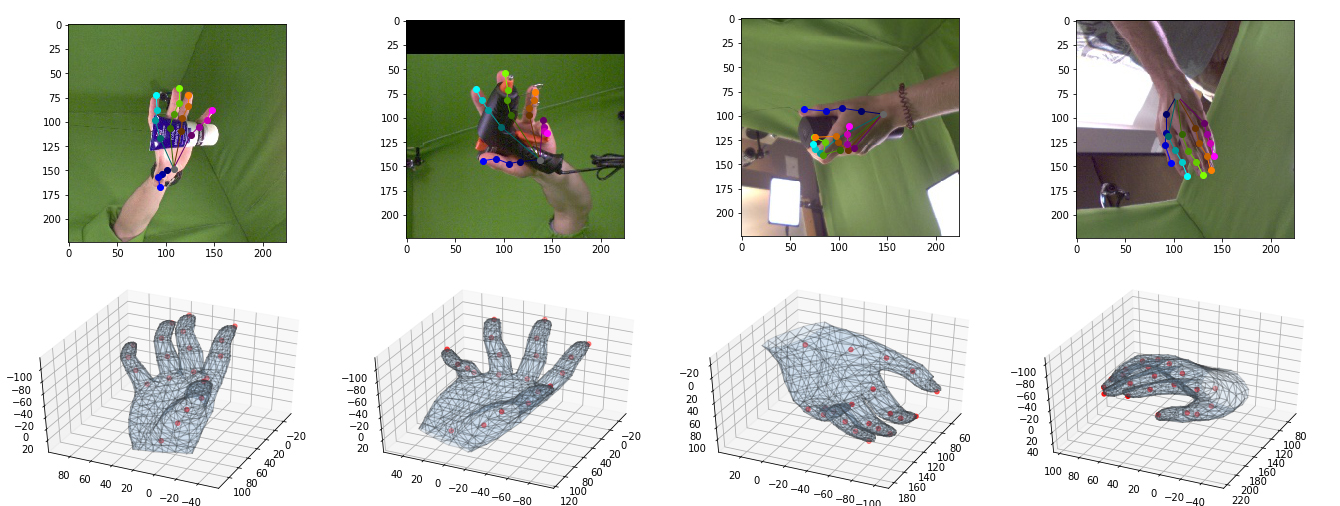
\includegraphics[width=1\textwidth]{fh}
\end{figure}

On Fig 4.1 we see accurate detection of key-point on Frei Hand Dataset. Even occluded points predicted on 2D and 3D. For instance, 3rd image from the left at Fig 4.1 show the accurate prediction of occluded little finger, which is seen at reflected reconstruction at the bottom.

\begin{figure}[H]
\caption{Examples of SynthHands\_A 3D reconstruction}
\centering
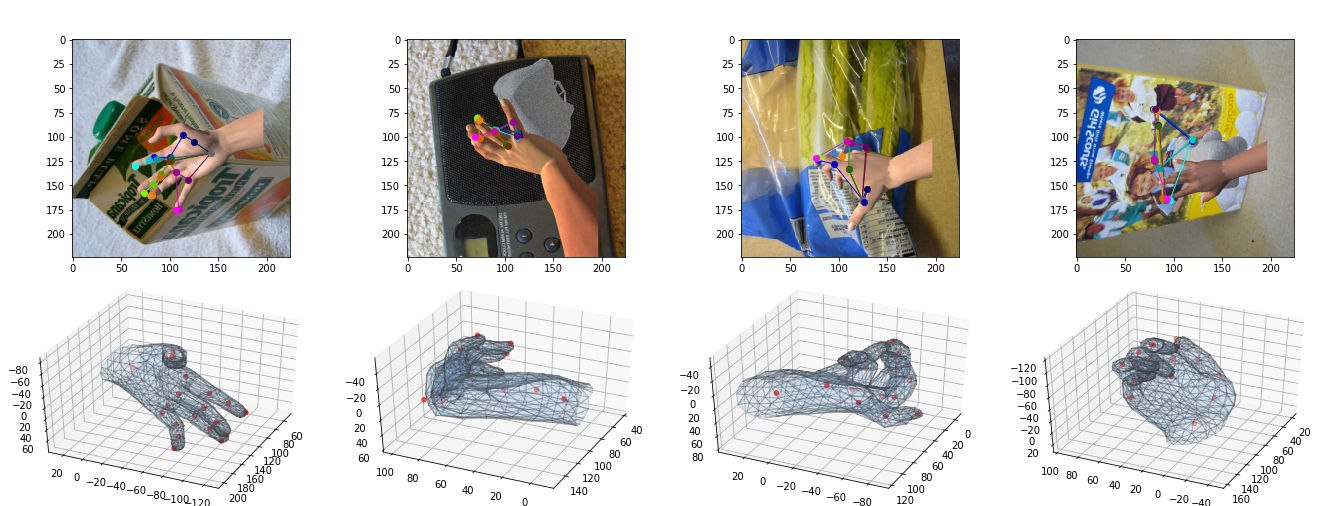
\includegraphics[width=1\textwidth]{sh_expls}
\end{figure}

In Fig 4.2 we see images from Synth Hand Dataset with an augmented background. The errors obtained on the SynthHands\_A dataset was the largest among all tests. Top images show a misdetection of 2D points. Now we can better understand a larger deviation of 3D model from 3D key-points detected by network AB\_PIC. Network C\_RNN estimates MANO parameters that encode some anatomy by design. The final shape it creates is more realistic than detected 3D points by AB\_PIC. 

\begin{figure}[H]
\caption{Examples of ASL 3D reconstruction}
\centering
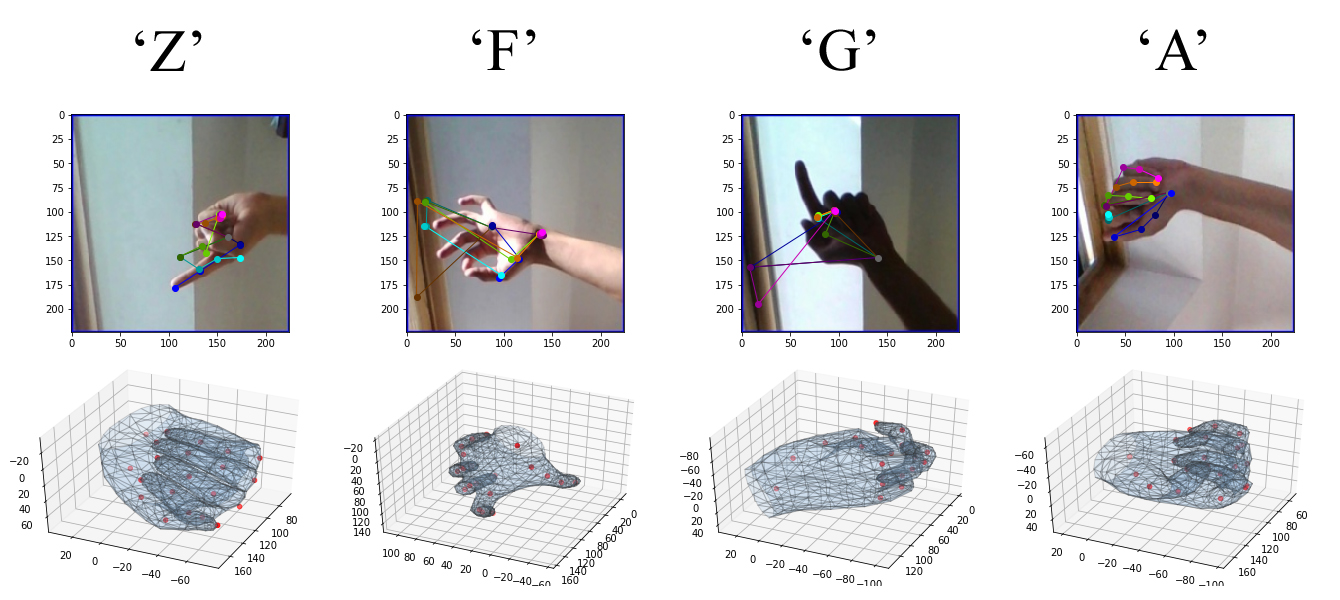
\includegraphics[width=1\textwidth]{alphabet}
\end{figure}

On Fig 4.3 we see predicted hand shapes for ASL. Most shapes mismatch originals. Even though in some cases, as for letter 'A' we see that the system can accurately reconstruct sign language pose. It is also a good example of how the final shape can fix misdetected points. 2D Key Points and depth were undetected on an index finger, but the final shape filled them to match the anatomy of the hand. 
\setcounter{mtc}{4}
\chapter{Conclusion}

Several architectures of neural networks were studied for the purpose of 3d hand shape reconstruction from video. It was shown that the addition of approximated hand positions at network input improves the quality of the final results. Also, it was observed that additional refinement of results is less efficient than the usage of extra annotated frames for both 2D key-point detection and depth estimation on all used datasets.

Also, a modular method for 3D shape estimation was introduced \cite{sys}. The method differs from the nearest known analog by RNN, which maps detected key-points to space of shape parameters. Method can be iteratively improved by making changes to certain parts and be adapted for 3D reconstruction from both photo and video sign language dictionaries. Implementation can be changed by the integration of architecture for a particular stage.

The selection of architecture for each stage heavily influences the quality of the reconstructed 3D hand shape. Although modular methods suffer from error accumulation, integration of networks that refine output from previous layers can help to overcome such performance degradation.

\vbox{%
\begin{description}
    \item[Achievements]
\end{description}
\begin{itemize}
\item Thesis introduces a method for hand shape parametrization.
\item Complete 3D hand shape reconstruction method from video sequences was developed, and its performance was studied with different ANN architectures based on UNET, STH, and introduced RNN.
\end{itemize}}

\section{Future work}

The next logical step would be to retrain the system on multiple datasets with data augmentation. After that, it needs to be compared with state of the art methods. Also, currently, the model does not distinguish between left and right hands and can not perform simultaneous detection of left and right hand. The integration of Part Affinity Fields can solve the limitation of single-hand detection \cite{PCP}. 

%----------------------------------------------------------------------------------------
%	THESIS CONTENT - APPENDICES
%----------------------------------------------------------------------------------------

\appendix % Cue to tell LaTeX that the following "chapters" are Appendices

% Include the appendices of the thesis as separate files from the Appendices folder
% Uncomment the lines as you write the Appendices

% 
\chapter{Code}

\section{Pseudocode}

Something on the topic



\endinput
%\include{Appendices/AppendixB}
%\include{Appendices/AppendixC}

%----------------------------------------------------------------------------------------
%	BIBLIOGRAPHY
%----------------------------------------------------------------------------------------

\printbibliography[heading=bibintoc]

%----------------------------------------------------------------------------------------

\end{document}  
